\AtBeginSection[]{
    \begin{frame}
        \setcounter{tocdepth}{1} % Show only sections
        \frametitle{Presentation Overview}
        \tableofcontents[currentsection]
    \end{frame}
}

\begin{frame}{Researcher Biography}
    \begin{columns}
        \column{0.5\textwidth}
            \begin{itemize}
                \item \textbf{Name: }Dave Figueroa
                \item \textbf{Grade:} M.Sc. Electronics Engineer, Federico Santa Maria Technical University (UTFSM), Valparaíso, Chile.
                \item \textbf{Research Interests:} AC microgrids, DC microgrids, partial power converters, vectorial control for AC machines drives and optimal control.
            \end{itemize}
        \column{0.5\textwidth}
            \begin{figure}
                \centering
                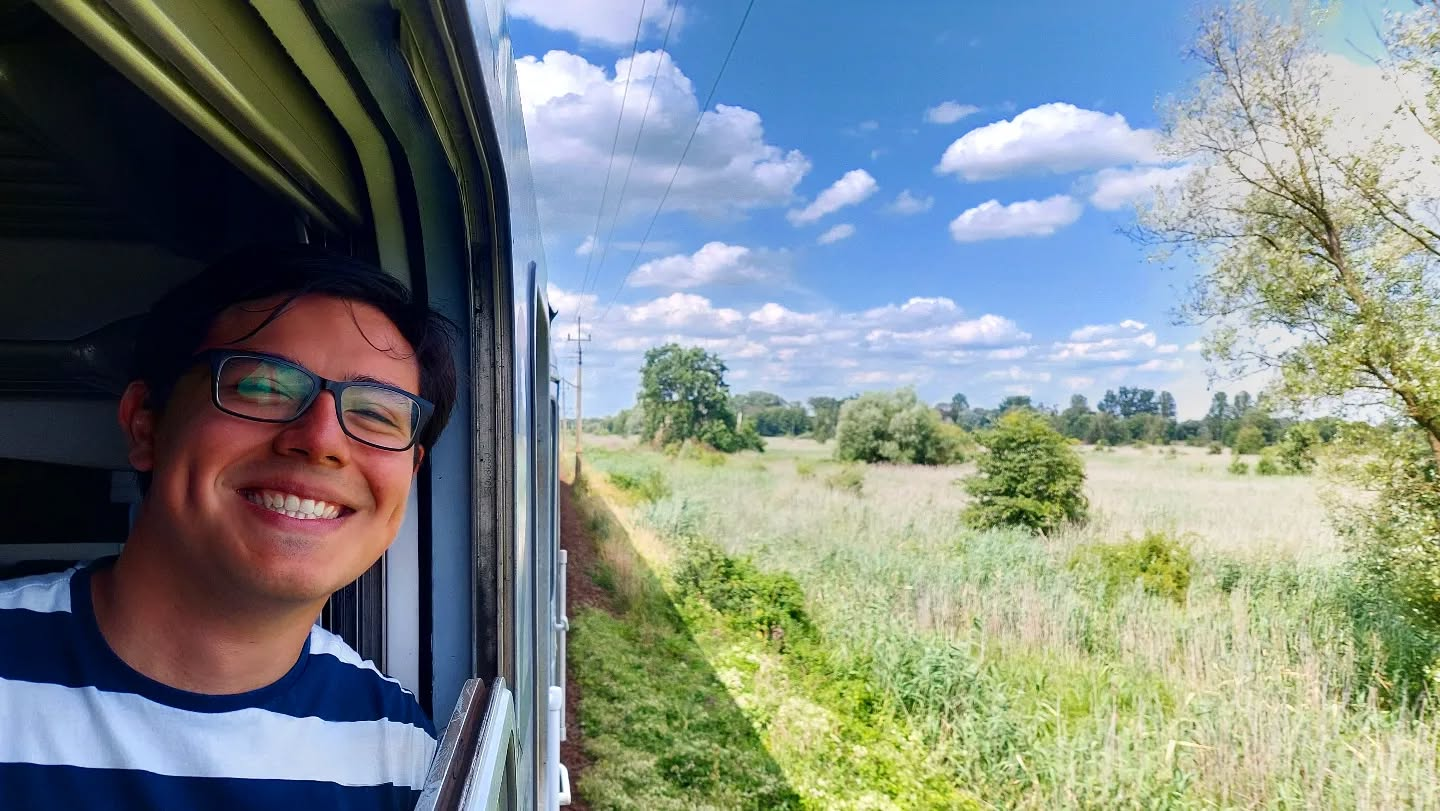
\includegraphics[width=\linewidth]{Images/Me.png}
            \end{figure}
    \end{columns}
\end{frame}

\begin{frame}{Researcher Biography (continued)}
    \begin{columns}
        \column{0.5\textwidth}
        \textbf{Education:}
            \begin{itemize}
                \item B.Sc Electronics Engineering
                \begin{itemize}
                    \item 2018 - 2022
                    \item UTFSM, Valparaíso, Chile
                \end{itemize}
                \item Curricular Exchange Program
                \begin{itemize}
                    \item February - July, 2023
                    \item Akademia Górtniczo Hutnicza, Kraków, Poland
                \end{itemize}
                \item M.Sc in Electronics Engineering
                \begin{itemize}
                    \item 2022 - 2024
                    \item UTFSM, Valparaíso, Chile
                \end{itemize}
            \end{itemize}
        \column{0.5\textwidth}
            \begin{figure}
                \centering
                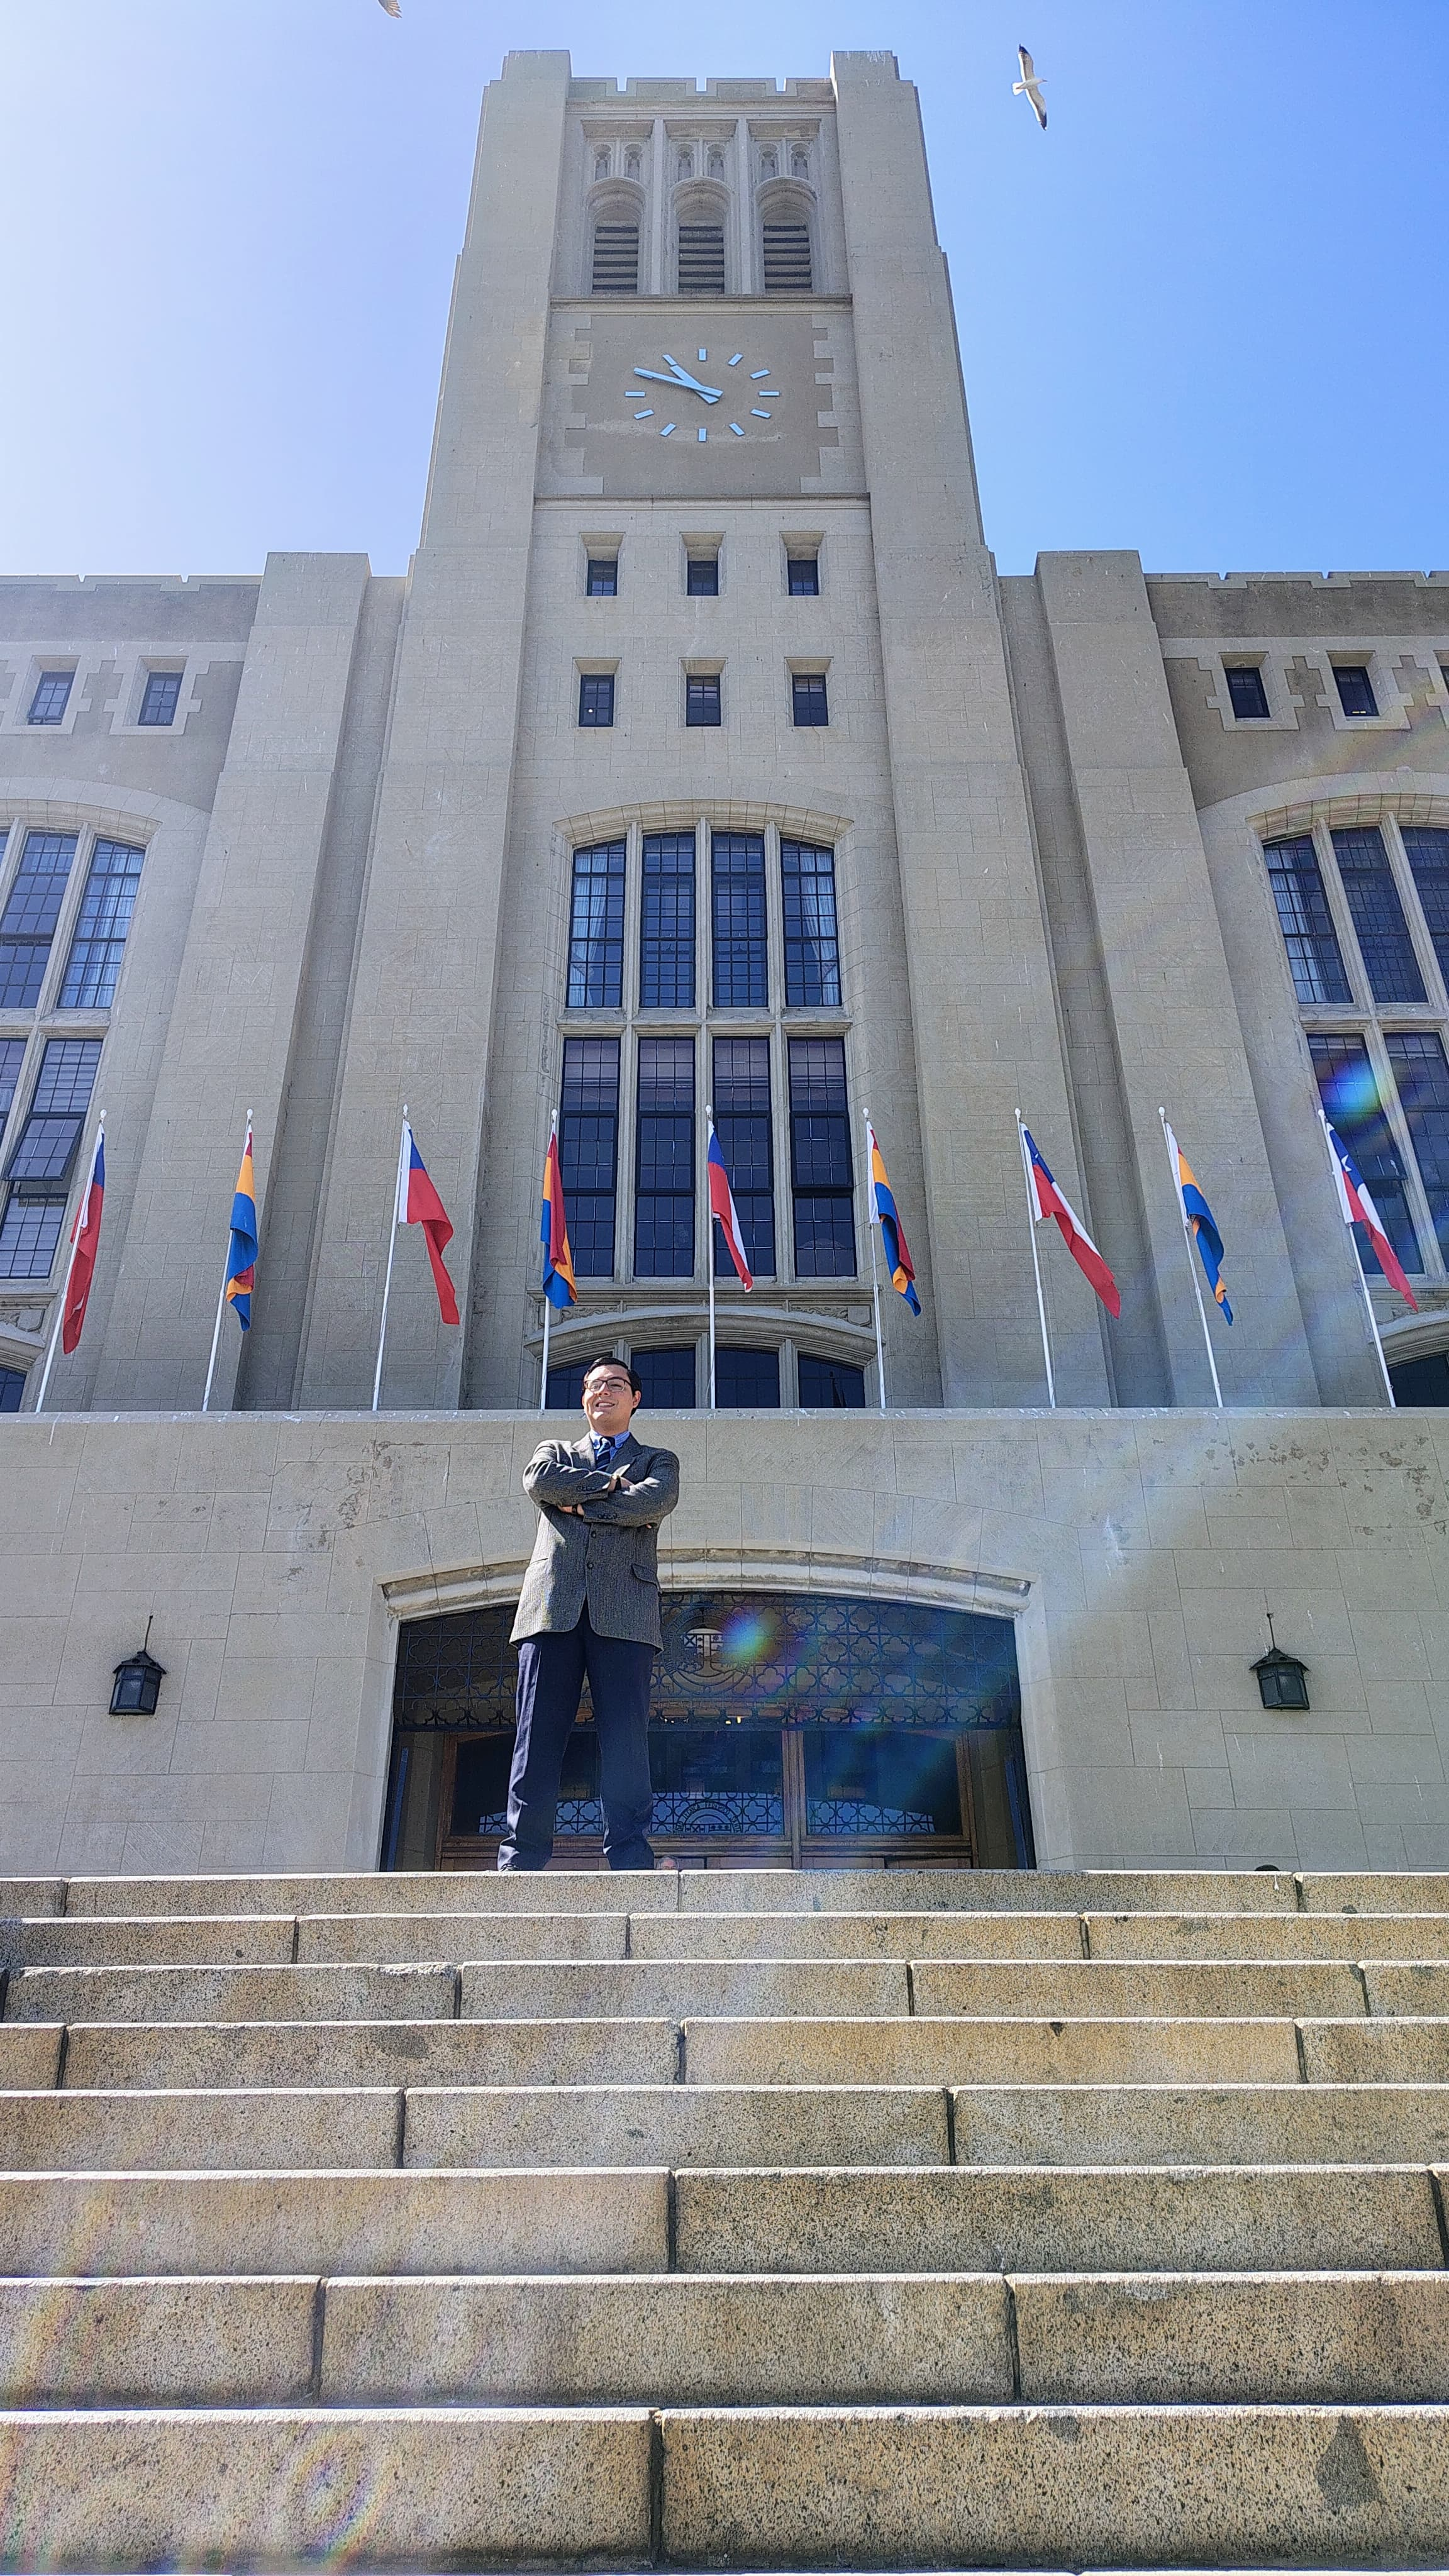
\includegraphics[width=0.5\linewidth]{Images/USM.jpg}
            \end{figure}
    \end{columns}
\end{frame}

\begin{frame}{Master's Thesis Topic}
    \begin{columns}
        \column{0.5\textwidth}
            \textbf{Model-based Predictive Control for a Grid-connected Distributed Energy Resource LCL Filter}\\
            Supervised by: \textit{Dr. César A. Silva}
            \begin{itemize}
                \item The goal was to achieve a primary control loop for a AC microgrid, capable of enforcing system constraints using MPC.
            \end{itemize}
        \column{0.5\textwidth}
            \begin{figure}
                \centering
                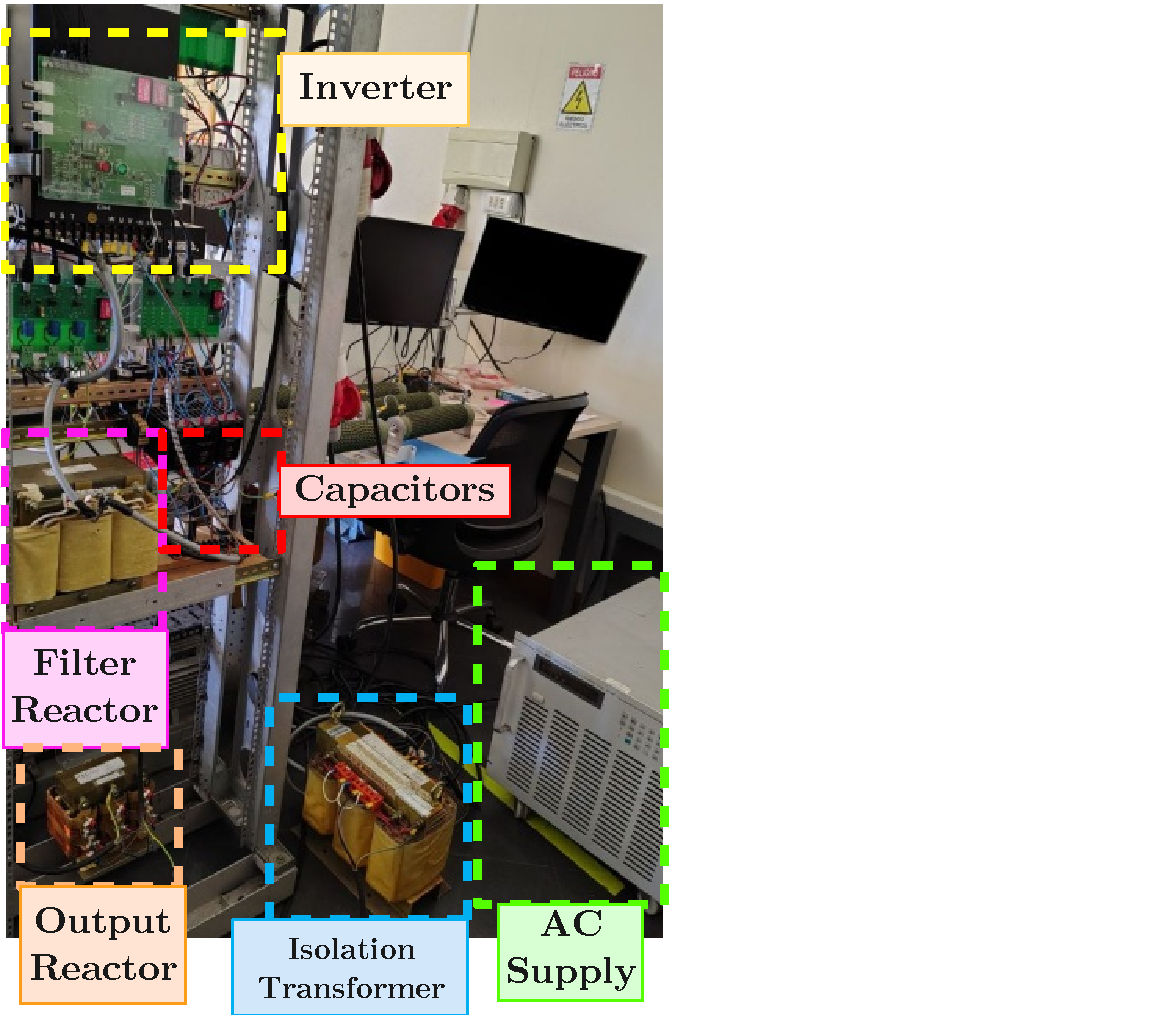
\includegraphics[width=0.6\linewidth]{Images/ExperimentalSetupEng.pdf}
            \end{figure}
    \end{columns}
\end{frame}

\begin{frame}{Master's Thesis Topic (continued)}
    \begin{columns}
        \column{0.5\textwidth}
            \textbf{Model-based Predictive Control for a Grid-connected Distributed Energy Resource LCL Filter}
            \begin{itemize}
                \item It employed the OSQP solver, which uses an ADMM optimization method.
                \item Experimental analysis of the primary control’s performance was presented, demonstrating that MPC control successfully limits the variables of interest.
            \end{itemize}
        \column{0.5\textwidth}
            \begin{figure}
                \centering
                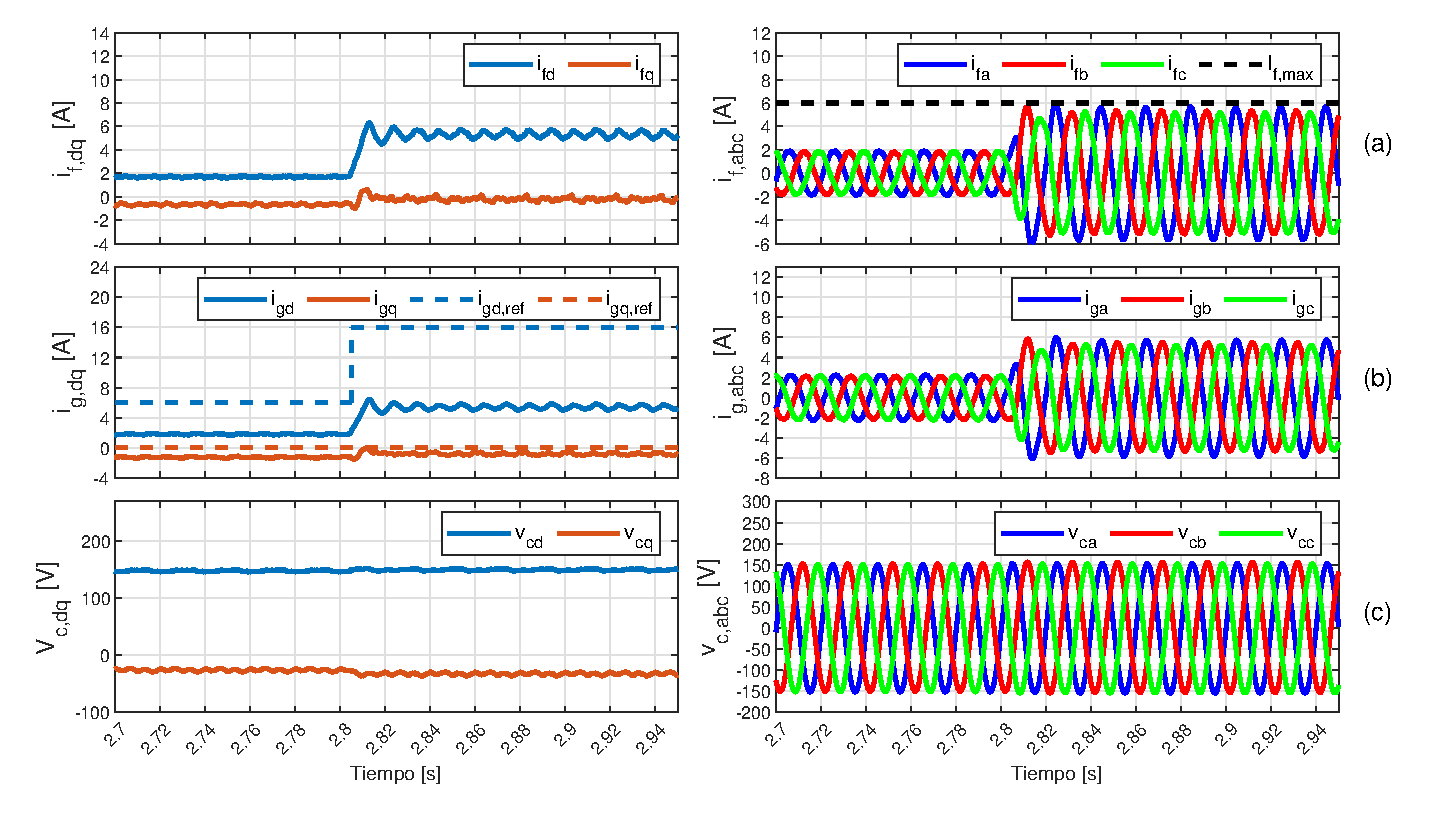
\includegraphics[width=1.1\linewidth]{Images/Variables_Exp_118.eps}
            \end{figure}
    \end{columns}
\end{frame}

\section{Introduction}
\begin{frame}{Problem of Interest}
    \begin{figure}
        \centering
        \resizebox{!}{4cm}{

\tikzset{every picture/.style={line width=0.75pt}} %set default line width to 0.75pt        

\begin{tikzpicture}[x=0.75pt,y=0.75pt,yscale=-1,xscale=1]
%uncomment if require: \path (0,137); %set diagram left start at 0, and has height of 137

%Shape: Rectangle [id:dp22623734830468978] 
\draw  [color={rgb, 255:red, 126; green, 211; blue, 33 }  ,draw opacity=1 ][fill={rgb, 255:red, 126; green, 211; blue, 33 }  ,fill opacity=0.25 ] (160,21) .. controls (160,18.24) and (162.24,16) .. (165,16) -- (203,16) .. controls (205.76,16) and (208,18.24) .. (208,21) -- (208,51) .. controls (208,53.76) and (205.76,56) .. (203,56) -- (165,56) .. controls (162.24,56) and (160,53.76) .. (160,51) -- cycle ;
%Shape: Rectangle [id:dp2708634841742097] 
\draw  [color={rgb, 255:red, 80; green, 227; blue, 194 }  ,draw opacity=1 ][fill={rgb, 255:red, 80; green, 227; blue, 194 }  ,fill opacity=0.25 ] (104,21) .. controls (104,18.24) and (106.24,16) .. (109,16) -- (147,16) .. controls (149.76,16) and (152,18.24) .. (152,21) -- (152,51) .. controls (152,53.76) and (149.76,56) .. (147,56) -- (109,56) .. controls (106.24,56) and (104,53.76) .. (104,51) -- cycle ;
%Shape: Rectangle [id:dp6625267657072971] 
\draw   (112,32) -- (144,32) -- (144,48) -- (112,48) -- cycle ;
%Shape: Rectangle [id:dp25871804946166965] 
\draw  [fill={rgb, 255:red, 0; green, 0; blue, 0 }  ,fill opacity=1 ] (114,30) -- (118,30) -- (118,32) -- (114,32) -- cycle ;
%Shape: Rectangle [id:dp842766551359059] 
\draw  [fill={rgb, 255:red, 0; green, 0; blue, 0 }  ,fill opacity=1 ] (138,30) -- (142,30) -- (142,32) -- (138,32) -- cycle ;
%Straight Lines [id:da20523841728231185] 
\draw    (114,36) -- (118,36) ;
%Straight Lines [id:da4965803158313489] 
\draw    (138,36) -- (142,36) ;
%Straight Lines [id:da16697029823961462] 
\draw    (140,34) -- (140,38) ;


%Shape: Rectangle [id:dp48496002666407567] 
\draw  [color={rgb, 255:red, 245; green, 166; blue, 35 }  ,draw opacity=1 ][fill={rgb, 255:red, 245; green, 166; blue, 35 }  ,fill opacity=0.25 ] (48,21) .. controls (48,18.24) and (50.24,16) .. (53,16) -- (91,16) .. controls (93.76,16) and (96,18.24) .. (96,21) -- (96,51) .. controls (96,53.76) and (93.76,56) .. (91,56) -- (53,56) .. controls (50.24,56) and (48,53.76) .. (48,51) -- cycle ;
%Shape: Parallelogram [id:dp6229021013770837] 
\draw  [fill={rgb, 255:red, 0; green, 0; blue, 255 }  ,fill opacity=0.25 ] (60.1,24) -- (92,24) -- (83.9,40) -- (52,40) -- cycle ;
%Straight Lines [id:da2873777946246239] 
\draw    (56,40) -- (60,32) ;
%Straight Lines [id:da7669514504697263] 
\draw    (60,40) -- (64,32) ;
%Straight Lines [id:da09929139384637531] 
\draw    (64,40) -- (68,32) ;
%Straight Lines [id:da8255108661997463] 
\draw    (68,40) -- (72,32) ;
%Straight Lines [id:da44066056373551565] 
\draw    (72,40) -- (76,32) ;
%Straight Lines [id:da5186395828464962] 
\draw    (76,40) -- (80,32) ;
%Straight Lines [id:da315764623168834] 
\draw    (80,40) -- (84,32) ;
%Straight Lines [id:da35552639471244163] 
\draw    (54,36) -- (86,36) ;
%Straight Lines [id:da8085339987485733] 
\draw    (60,32) -- (64,24) ;
%Straight Lines [id:da9522346734197424] 
\draw    (64,32) -- (68,24) ;
%Straight Lines [id:da21961176628582213] 
\draw    (68,32) -- (72,24) ;
%Straight Lines [id:da1185914033172557] 
\draw    (72,32) -- (76,24) ;
%Straight Lines [id:da007154677041725899] 
\draw    (76,32) -- (80,24) ;
%Straight Lines [id:da30851582505063013] 
\draw    (80,32) -- (84,24) ;
%Straight Lines [id:da8633681024285915] 
\draw    (84,32) -- (88,24) ;
%Straight Lines [id:da06294065895051859] 
\draw    (58,28) -- (90,28) ;
%Shape: Rectangle [id:dp5442302554358358] 
\draw  [fill={rgb, 255:red, 0; green, 0; blue, 0 }  ,fill opacity=1 ] (60,46) -- (84,46) -- (84,48) -- (60,48) -- cycle ;
%Shape: Rectangle [id:dp20057972152279535] 
\draw  [fill={rgb, 255:red, 0; green, 0; blue, 0 }  ,fill opacity=1 ] (70,40) -- (74,40) -- (74,46) -- (70,46) -- cycle ;
%Straight Lines [id:da2916294274108977] 
\draw    (56,32) -- (88,32) ;

%Shape: Rectangle [id:dp3951771829324371] 
\draw  [fill={rgb, 255:red, 255; green, 255; blue, 255 }  ,fill opacity=1 ][general shadow={fill=black,shadow xshift=0.75pt,shadow yshift=-0.75pt}] (55.85,64.53) -- (88,64.53) -- (88,96) -- (55.85,96) -- cycle ;
%Straight Lines [id:da3481313771128698] 
\draw    (88,64) -- (55.85,97.3) ;

%Straight Lines [id:da9870292125997671] 
\draw [line width=2.25]    (40,112) -- (216,112) ;
%Shape: Ellipse [id:dp6838425524961658] 
\draw   (16.7,112) .. controls (16.7,105.37) and (21.91,100) .. (28.35,100) .. controls (34.78,100) and (40,105.37) .. (40,112) .. controls (40,118.63) and (34.78,124) .. (28.35,124) .. controls (21.91,124) and (16.7,118.63) .. (16.7,112) -- cycle ;
%Curve Lines [id:da37851557635969724] 
\draw    (21.32,111.26) .. controls (28.16,92.78) and (26.5,128.78) .. (35.01,111.64) ;

%Straight Lines [id:da39937420126132706] 
\draw    (72,56) -- (72,64) ;
%Shape: Rectangle [id:dp6107823240243895] 
\draw  [fill={rgb, 255:red, 255; green, 255; blue, 255 }  ,fill opacity=1 ][general shadow={fill=black,shadow xshift=0.75pt,shadow yshift=-0.75pt}] (112,64.53) -- (144.15,64.53) -- (144.15,96) -- (112,96) -- cycle ;
%Straight Lines [id:da09617220369365054] 
\draw    (144.15,64) -- (112,97.3) ;

%Straight Lines [id:da739431614032469] 
\draw    (128,56) -- (128,64) ;
%Straight Lines [id:da944762266663753] 
\draw    (72,96) -- (72,112) ;
\draw [shift={(72,112)}, rotate = 90] [color={rgb, 255:red, 0; green, 0; blue, 0 }  ][fill={rgb, 255:red, 0; green, 0; blue, 0 }  ][line width=0.75]      (0, 0) circle [x radius= 2.01, y radius= 2.01]   ;
%Straight Lines [id:da31010194804850544] 
\draw    (128,96) -- (128,112) ;
\draw [shift={(128,112)}, rotate = 90] [color={rgb, 255:red, 0; green, 0; blue, 0 }  ][fill={rgb, 255:red, 0; green, 0; blue, 0 }  ][line width=0.75]      (0, 0) circle [x radius= 2.01, y radius= 2.01]   ;
%Shape: Path Data [id:dp3159470169843912] 
\draw  [fill={rgb, 255:red, 245; green, 166; blue, 35 }  ,fill opacity=0.25 ] (200,48) -- (188,48) -- (188,40) -- (180,40) -- (180,48) -- (168,48) -- (168,32) -- (184,24) -- (200,32) -- (200,48) -- cycle ;
%Straight Lines [id:da6494885780264399] 
\draw    (164,32) -- (184,22) ;
%Straight Lines [id:da2725982309448327] 
\draw    (184,22) -- (204,32) ;
%Shape: Rectangle [id:dp7306207830653915] 
\draw  [fill={rgb, 255:red, 0; green, 0; blue, 0 }  ,fill opacity=1 ] (196,24) -- (198,24) -- (198,30) -- (196,30) -- cycle ;

%Straight Lines [id:da6572081669980756] 
\draw    (184,56) -- (184,112) ;
\draw [shift={(184,112)}, rotate = 90] [color={rgb, 255:red, 0; green, 0; blue, 0 }  ][fill={rgb, 255:red, 0; green, 0; blue, 0 }  ][line width=0.75]      (0, 0) circle [x radius= 2.01, y radius= 2.01]   ;

% Text Node
\draw (28,92.5) node  [font=\scriptsize] [align=left] {LV-AC};
% Text Node
\draw (65.5,71.5) node  [font=\scriptsize] [align=left] {DC};
% Text Node
\draw (78.5,88.5) node  [font=\scriptsize] [align=left] {AC};
% Text Node
\draw (134.65,88.5) node  [font=\scriptsize] [align=left] {AC};
% Text Node
\draw (121.65,71.5) node  [font=\scriptsize] [align=left] {DC};
% Text Node
\draw (128.5,120.5) node  [font=\scriptsize] [align=left] {AC Microgrid};
% Text Node
\draw (73,8.5) node  [font=\scriptsize] [align=left] {PV};
% Text Node
\draw (128,8.5) node  [font=\scriptsize] [align=left] {BESS};
% Text Node
\draw (184,8.5) node  [font=\scriptsize] [align=left] {AC Loads};


\end{tikzpicture}}
        \caption{An AC microgrid connected to a LV-AC grid.}
    \end{figure}
\end{frame}

\begin{frame}{Problem of Interest (continued)}
    \begin{figure}
        \centering
        \resizebox{!}{4cm}{

\tikzset{every picture/.style={line width=0.75pt}} %set default line width to 0.75pt        

\begin{tikzpicture}[x=0.75pt,y=0.75pt,yscale=-1,xscale=1]
%uncomment if require: \path (0,137); %set diagram left start at 0, and has height of 137

%Shape: Rectangle [id:dp6882500997417098] 
\draw  [color={rgb, 255:red, 126; green, 211; blue, 33 }  ,draw opacity=1 ][fill={rgb, 255:red, 126; green, 211; blue, 33 }  ,fill opacity=0.25 ] (160,21) .. controls (160,18.24) and (162.24,16) .. (165,16) -- (203,16) .. controls (205.76,16) and (208,18.24) .. (208,21) -- (208,51) .. controls (208,53.76) and (205.76,56) .. (203,56) -- (165,56) .. controls (162.24,56) and (160,53.76) .. (160,51) -- cycle ;
%Shape: Circle [id:dp032812107775992194] 
\draw   (166,30) .. controls (166,26.69) and (168.69,24) .. (172,24) .. controls (175.31,24) and (178,26.69) .. (178,30) .. controls (178,33.31) and (175.31,36) .. (172,36) .. controls (168.69,36) and (166,33.31) .. (166,30) -- cycle ;
%Shape: Circle [id:dp9262085288187545] 
\draw   (168,29) .. controls (168,28.45) and (168.45,28) .. (169,28) .. controls (169.55,28) and (170,28.45) .. (170,29) .. controls (170,29.55) and (169.55,30) .. (169,30) .. controls (168.45,30) and (168,29.55) .. (168,29) -- cycle ;
%Shape: Circle [id:dp6448495688072267] 
\draw   (174,29) .. controls (174,28.45) and (174.45,28) .. (175,28) .. controls (175.55,28) and (176,28.45) .. (176,29) .. controls (176,29.55) and (175.55,30) .. (175,30) .. controls (174.45,30) and (174,29.55) .. (174,29) -- cycle ;
%Shape: Circle [id:dp41636039438594974] 
\draw   (171,33) .. controls (171,32.45) and (171.45,32) .. (172,32) .. controls (172.55,32) and (173,32.45) .. (173,33) .. controls (173,33.55) and (172.55,34) .. (172,34) .. controls (171.45,34) and (171,33.55) .. (171,33) -- cycle ;

%Shape: Rectangle [id:dp42253209047103657] 
\draw   (184,24) -- (200,24) -- (200,48) -- (184,48) -- cycle ;
%Curve Lines [id:da6018278864986624] 
\draw    (172,36) .. controls (169.25,46.92) and (180.45,53.69) .. (184,32) ;
%Shape: Rectangle [id:dp6239868893891705] 
\draw  [fill={rgb, 255:red, 155; green, 155; blue, 155 }  ,fill opacity=1 ] (170,36) -- (174,36) -- (174,42) -- (170,42) -- cycle ;
%Shape: Rectangle [id:dp8196162974902845] 
\draw  [fill={rgb, 255:red, 255; green, 0; blue, 0 }  ,fill opacity=0.25 ] (186,26) -- (198,26) -- (198,32) -- (186,32) -- cycle ;

%Shape: Rectangle [id:dp5110058203946946] 
\draw  [color={rgb, 255:red, 80; green, 227; blue, 194 }  ,draw opacity=1 ][fill={rgb, 255:red, 80; green, 227; blue, 194 }  ,fill opacity=0.25 ] (104,21) .. controls (104,18.24) and (106.24,16) .. (109,16) -- (147,16) .. controls (149.76,16) and (152,18.24) .. (152,21) -- (152,51) .. controls (152,53.76) and (149.76,56) .. (147,56) -- (109,56) .. controls (106.24,56) and (104,53.76) .. (104,51) -- cycle ;
%Shape: Rectangle [id:dp9159046267117186] 
\draw   (112,32) -- (144,32) -- (144,48) -- (112,48) -- cycle ;
%Shape: Rectangle [id:dp17388466684389203] 
\draw  [fill={rgb, 255:red, 0; green, 0; blue, 0 }  ,fill opacity=1 ] (114,30) -- (118,30) -- (118,32) -- (114,32) -- cycle ;
%Shape: Rectangle [id:dp21761452467577969] 
\draw  [fill={rgb, 255:red, 0; green, 0; blue, 0 }  ,fill opacity=1 ] (138,30) -- (142,30) -- (142,32) -- (138,32) -- cycle ;
%Straight Lines [id:da860877487496249] 
\draw    (114,36) -- (118,36) ;
%Straight Lines [id:da0002607012984467971] 
\draw    (138,36) -- (142,36) ;
%Straight Lines [id:da14790630046288955] 
\draw    (140,34) -- (140,38) ;


%Shape: Rectangle [id:dp8223061284418032] 
\draw  [color={rgb, 255:red, 245; green, 166; blue, 35 }  ,draw opacity=1 ][fill={rgb, 255:red, 245; green, 166; blue, 35 }  ,fill opacity=0.25 ] (48,21) .. controls (48,18.24) and (50.24,16) .. (53,16) -- (91,16) .. controls (93.76,16) and (96,18.24) .. (96,21) -- (96,51) .. controls (96,53.76) and (93.76,56) .. (91,56) -- (53,56) .. controls (50.24,56) and (48,53.76) .. (48,51) -- cycle ;
%Shape: Parallelogram [id:dp5784515690514784] 
\draw  [fill={rgb, 255:red, 0; green, 0; blue, 255 }  ,fill opacity=0.25 ] (60.1,24) -- (92,24) -- (83.9,40) -- (52,40) -- cycle ;
%Straight Lines [id:da7724685088462382] 
\draw    (56,40) -- (60,32) ;
%Straight Lines [id:da6858521691777979] 
\draw    (60,40) -- (64,32) ;
%Straight Lines [id:da08367305959077243] 
\draw    (64,40) -- (68,32) ;
%Straight Lines [id:da8984419540494084] 
\draw    (68,40) -- (72,32) ;
%Straight Lines [id:da1470230625871407] 
\draw    (72,40) -- (76,32) ;
%Straight Lines [id:da7283185095592601] 
\draw    (76,40) -- (80,32) ;
%Straight Lines [id:da6436428106786771] 
\draw    (80,40) -- (84,32) ;
%Straight Lines [id:da0641437838156087] 
\draw    (54,36) -- (86,36) ;
%Straight Lines [id:da5951523990184908] 
\draw    (60,32) -- (64,24) ;
%Straight Lines [id:da7366464383172375] 
\draw    (64,32) -- (68,24) ;
%Straight Lines [id:da8981156056502326] 
\draw    (68,32) -- (72,24) ;
%Straight Lines [id:da8014733289952307] 
\draw    (72,32) -- (76,24) ;
%Straight Lines [id:da46472076987328315] 
\draw    (76,32) -- (80,24) ;
%Straight Lines [id:da015194263413285558] 
\draw    (80,32) -- (84,24) ;
%Straight Lines [id:da9605301026918074] 
\draw    (84,32) -- (88,24) ;
%Straight Lines [id:da8532252518526424] 
\draw    (58,28) -- (90,28) ;
%Shape: Rectangle [id:dp2187517991000938] 
\draw  [fill={rgb, 255:red, 0; green, 0; blue, 0 }  ,fill opacity=1 ] (60,46) -- (84,46) -- (84,48) -- (60,48) -- cycle ;
%Shape: Rectangle [id:dp6224356280789016] 
\draw  [fill={rgb, 255:red, 0; green, 0; blue, 0 }  ,fill opacity=1 ] (70,40) -- (74,40) -- (74,46) -- (70,46) -- cycle ;
%Straight Lines [id:da6926506860294483] 
\draw    (56,32) -- (88,32) ;

%Shape: Rectangle [id:dp4544479503646166] 
\draw  [fill={rgb, 255:red, 255; green, 255; blue, 255 }  ,fill opacity=1 ][general shadow={fill=black,shadow xshift=0.75pt,shadow yshift=-0.75pt}] (55.85,64.53) -- (88,64.53) -- (88,96) -- (55.85,96) -- cycle ;
%Straight Lines [id:da867110354326456] 
\draw    (88,64) -- (55.85,97.3) ;

%Straight Lines [id:da22950679417781106] 
\draw [line width=2.25]    (40,112) -- (216,112) ;
%Shape: Ellipse [id:dp8041305172491726] 
\draw   (16.7,112) .. controls (16.7,105.37) and (21.91,100) .. (28.35,100) .. controls (34.78,100) and (40,105.37) .. (40,112) .. controls (40,118.63) and (34.78,124) .. (28.35,124) .. controls (21.91,124) and (16.7,118.63) .. (16.7,112) -- cycle ;
%Straight Lines [id:da3644680042373436] 
\draw    (72,56) -- (72,64) ;
%Shape: Rectangle [id:dp2798141303683963] 
\draw  [fill={rgb, 255:red, 255; green, 255; blue, 255 }  ,fill opacity=1 ][general shadow={fill=black,shadow xshift=0.75pt,shadow yshift=-0.75pt}] (112,64.53) -- (144.15,64.53) -- (144.15,96) -- (112,96) -- cycle ;
%Straight Lines [id:da8481766623987883] 
\draw    (144.15,64) -- (112,97.3) ;

%Straight Lines [id:da4333393270239132] 
\draw    (128,56) -- (128,64) ;
%Straight Lines [id:da8098457488359423] 
\draw    (72,96) -- (72,112) ;
\draw [shift={(72,112)}, rotate = 90] [color={rgb, 255:red, 0; green, 0; blue, 0 }  ][fill={rgb, 255:red, 0; green, 0; blue, 0 }  ][line width=0.75]      (0, 0) circle [x radius= 2.01, y radius= 2.01]   ;
%Straight Lines [id:da11337801661893732] 
\draw    (128,96) -- (128,112) ;
\draw [shift={(128,112)}, rotate = 90] [color={rgb, 255:red, 0; green, 0; blue, 0 }  ][fill={rgb, 255:red, 0; green, 0; blue, 0 }  ][line width=0.75]      (0, 0) circle [x radius= 2.01, y radius= 2.01]   ;
%Straight Lines [id:da4688791529860943] 
\draw    (184,96) -- (184,112) ;
\draw [shift={(184,112)}, rotate = 90] [color={rgb, 255:red, 0; green, 0; blue, 0 }  ][fill={rgb, 255:red, 0; green, 0; blue, 0 }  ][line width=0.75]      (0, 0) circle [x radius= 2.01, y radius= 2.01]   ;
%Shape: Rectangle [id:dp0025991773379798744] 
\draw  [fill={rgb, 255:red, 255; green, 255; blue, 255 }  ,fill opacity=1 ][general shadow={fill=black,shadow xshift=0.75pt,shadow yshift=-0.75pt}] (167.85,63.23) -- (200,63.23) -- (200,94.7) -- (167.85,94.7) -- cycle ;
%Straight Lines [id:da5759364710881532] 
\draw    (200,62.7) -- (167.85,96) ;

%Straight Lines [id:da5233375145007366] 
\draw    (184,56) -- (184,64) ;

% Text Node
\draw (28,92.5) node  [font=\scriptsize] [align=left] {LV-DC};
% Text Node
\draw (65.5,71.5) node  [font=\scriptsize] [align=left] {DC};
% Text Node
\draw (78.5,88.5) node  [font=\scriptsize] [align=left] {DC};
% Text Node
\draw (134.65,88.5) node  [font=\scriptsize] [align=left] {DC};
% Text Node
\draw (121.65,71.5) node  [font=\scriptsize] [align=left] {DC};
% Text Node
\draw (128.5,120.5) node  [font=\scriptsize] [align=left] {DC Microgrid};
% Text Node
\draw (190.5,87.2) node  [font=\scriptsize] [align=left] {DC};
% Text Node
\draw (177.5,70.2) node  [font=\scriptsize] [align=left] {DC};
% Text Node
\draw (72,8.5) node  [font=\scriptsize] [align=left] {PV};
% Text Node
\draw (128,8.5) node  [font=\scriptsize] [align=left] {BESS};
% Text Node
\draw (184,8.5) node  [font=\scriptsize] [align=left] {EV Chargers};
% Text Node
\draw (8.5,102) node    {$+$};


\end{tikzpicture}}
        \caption{A DC microgrid.}
    \end{figure}
\end{frame}

\begin{frame}{Problem of Interest: Integration of AC and DC Microgrids}
    \begin{figure}
        \centering
        \resizebox{!}{5.3cm}{

\tikzset{every picture/.style={line width=0.75pt}} %set default line width to 0.75pt        

\begin{tikzpicture}[x=0.75pt,y=0.75pt,yscale=-1,xscale=1]
%uncomment if require: \path (0,315); %set diagram left start at 0, and has height of 315

%Shape: Rectangle [id:dp35532886431683575] 
\draw  [color={rgb, 255:red, 255; green, 0; blue, 0 }  ,draw opacity=1 ][fill={rgb, 255:red, 255; green, 0; blue, 0 }  ,fill opacity=0.25 ][dash pattern={on 4.5pt off 4.5pt}] (88,133) .. controls (88,130.24) and (90.24,128) .. (93,128) -- (187,128) .. controls (189.76,128) and (192,130.24) .. (192,133) -- (192,171) .. controls (192,173.76) and (189.76,176) .. (187,176) -- (93,176) .. controls (90.24,176) and (88,173.76) .. (88,171) -- cycle ;
%Shape: Rectangle [id:dp0086710224164257] 
\draw  [color={rgb, 255:red, 126; green, 211; blue, 33 }  ,draw opacity=1 ][fill={rgb, 255:red, 126; green, 211; blue, 33 }  ,fill opacity=0.25 ] (200,21) .. controls (200,18.24) and (202.24,16) .. (205,16) -- (243,16) .. controls (245.76,16) and (248,18.24) .. (248,21) -- (248,51) .. controls (248,53.76) and (245.76,56) .. (243,56) -- (205,56) .. controls (202.24,56) and (200,53.76) .. (200,51) -- cycle ;
%Shape: Rectangle [id:dp05031174656890136] 
\draw  [color={rgb, 255:red, 80; green, 227; blue, 194 }  ,draw opacity=1 ][fill={rgb, 255:red, 80; green, 227; blue, 194 }  ,fill opacity=0.25 ] (144,21) .. controls (144,18.24) and (146.24,16) .. (149,16) -- (187,16) .. controls (189.76,16) and (192,18.24) .. (192,21) -- (192,51) .. controls (192,53.76) and (189.76,56) .. (187,56) -- (149,56) .. controls (146.24,56) and (144,53.76) .. (144,51) -- cycle ;
%Shape: Rectangle [id:dp6308344152321033] 
\draw   (152,32) -- (184,32) -- (184,48) -- (152,48) -- cycle ;
%Shape: Rectangle [id:dp2519084009436485] 
\draw  [fill={rgb, 255:red, 0; green, 0; blue, 0 }  ,fill opacity=1 ] (154,30) -- (158,30) -- (158,32) -- (154,32) -- cycle ;
%Shape: Rectangle [id:dp7947750289265254] 
\draw  [fill={rgb, 255:red, 0; green, 0; blue, 0 }  ,fill opacity=1 ] (178,30) -- (182,30) -- (182,32) -- (178,32) -- cycle ;
%Straight Lines [id:da022849387871711313] 
\draw    (154,36) -- (158,36) ;
%Straight Lines [id:da8843959778472783] 
\draw    (178,36) -- (182,36) ;
%Straight Lines [id:da14682611923607514] 
\draw    (180,34) -- (180,38) ;


%Shape: Rectangle [id:dp01617760227064724] 
\draw  [color={rgb, 255:red, 245; green, 166; blue, 35 }  ,draw opacity=1 ][fill={rgb, 255:red, 245; green, 166; blue, 35 }  ,fill opacity=0.25 ] (88,21) .. controls (88,18.24) and (90.24,16) .. (93,16) -- (131,16) .. controls (133.76,16) and (136,18.24) .. (136,21) -- (136,51) .. controls (136,53.76) and (133.76,56) .. (131,56) -- (93,56) .. controls (90.24,56) and (88,53.76) .. (88,51) -- cycle ;
%Shape: Parallelogram [id:dp7249897775938421] 
\draw  [fill={rgb, 255:red, 0; green, 0; blue, 255 }  ,fill opacity=0.25 ] (100.1,24) -- (132,24) -- (123.9,40) -- (92,40) -- cycle ;
%Straight Lines [id:da044669355651341114] 
\draw    (96,40) -- (100,32) ;
%Straight Lines [id:da8109059917629575] 
\draw    (100,40) -- (104,32) ;
%Straight Lines [id:da5908989104168503] 
\draw    (104,40) -- (108,32) ;
%Straight Lines [id:da8590136185427117] 
\draw    (108,40) -- (112,32) ;
%Straight Lines [id:da6389775198064604] 
\draw    (112,40) -- (116,32) ;
%Straight Lines [id:da23494127595306402] 
\draw    (116,40) -- (120,32) ;
%Straight Lines [id:da0909227770605665] 
\draw    (120,40) -- (124,32) ;
%Straight Lines [id:da053988832372001916] 
\draw    (94,36) -- (126,36) ;
%Straight Lines [id:da23061586991599592] 
\draw    (100,32) -- (104,24) ;
%Straight Lines [id:da45676079495353794] 
\draw    (104,32) -- (108,24) ;
%Straight Lines [id:da3657894219570965] 
\draw    (108,32) -- (112,24) ;
%Straight Lines [id:da014790554769904318] 
\draw    (112,32) -- (116,24) ;
%Straight Lines [id:da6329138262294458] 
\draw    (116,32) -- (120,24) ;
%Straight Lines [id:da013400153550848337] 
\draw    (120,32) -- (124,24) ;
%Straight Lines [id:da8438401787664913] 
\draw    (124,32) -- (128,24) ;
%Straight Lines [id:da6571996749071958] 
\draw    (98,28) -- (130,28) ;
%Shape: Rectangle [id:dp7890702161156278] 
\draw  [fill={rgb, 255:red, 0; green, 0; blue, 0 }  ,fill opacity=1 ] (100,46) -- (124,46) -- (124,48) -- (100,48) -- cycle ;
%Shape: Rectangle [id:dp043107439399324265] 
\draw  [fill={rgb, 255:red, 0; green, 0; blue, 0 }  ,fill opacity=1 ] (110,40) -- (114,40) -- (114,46) -- (110,46) -- cycle ;
%Straight Lines [id:da6464411488066013] 
\draw    (96,32) -- (128,32) ;

%Shape: Rectangle [id:dp09509095756390362] 
\draw  [fill={rgb, 255:red, 255; green, 255; blue, 255 }  ,fill opacity=1 ][general shadow={fill=black,shadow xshift=0.75pt,shadow yshift=-0.75pt}] (95.85,64.53) -- (128,64.53) -- (128,96) -- (95.85,96) -- cycle ;
%Straight Lines [id:da7658272557907531] 
\draw    (128,64) -- (95.85,97.3) ;

%Straight Lines [id:da3193204246819088] 
\draw [line width=2.25]    (72,112) -- (256,112) ;
%Shape: Ellipse [id:dp17506684300684738] 
\draw   (9,112) .. controls (9,105.37) and (14.22,100) .. (20.65,100) .. controls (27.09,100) and (32.3,105.37) .. (32.3,112) .. controls (32.3,118.63) and (27.09,124) .. (20.65,124) .. controls (14.22,124) and (9,118.63) .. (9,112) -- cycle ;
%Curve Lines [id:da5154233932953838] 
\draw    (13.62,111.26) .. controls (20.47,92.78) and (18.8,128.78) .. (27.31,111.64) ;

%Straight Lines [id:da7946987619267307] 
\draw    (112,56) -- (112,64) ;
%Shape: Rectangle [id:dp09111719877291558] 
\draw  [fill={rgb, 255:red, 255; green, 255; blue, 255 }  ,fill opacity=1 ][general shadow={fill=black,shadow xshift=0.75pt,shadow yshift=-0.75pt}] (152,64.53) -- (184.15,64.53) -- (184.15,96) -- (152,96) -- cycle ;
%Straight Lines [id:da815440705910415] 
\draw    (184.15,64) -- (152,97.3) ;

%Straight Lines [id:da8344835851517192] 
\draw    (168,56) -- (168,64) ;
%Straight Lines [id:da8709837915701788] 
\draw    (112,96) -- (112,112) ;
\draw [shift={(112,112)}, rotate = 90] [color={rgb, 255:red, 0; green, 0; blue, 0 }  ][fill={rgb, 255:red, 0; green, 0; blue, 0 }  ][line width=0.75]      (0, 0) circle [x radius= 2.01, y radius= 2.01]   ;
%Straight Lines [id:da3456223398148759] 
\draw    (168,96) -- (168,112) ;
\draw [shift={(168,112)}, rotate = 90] [color={rgb, 255:red, 0; green, 0; blue, 0 }  ][fill={rgb, 255:red, 0; green, 0; blue, 0 }  ][line width=0.75]      (0, 0) circle [x radius= 2.01, y radius= 2.01]   ;
%Shape: Path Data [id:dp8852492192465802] 
\draw  [fill={rgb, 255:red, 245; green, 166; blue, 35 }  ,fill opacity=0.25 ] (240,48) -- (228,48) -- (228,40) -- (220,40) -- (220,48) -- (208,48) -- (208,32) -- (224,24) -- (240,32) -- (240,48) -- cycle ;
%Straight Lines [id:da5531820633243698] 
\draw    (204,32) -- (224,22) ;
%Straight Lines [id:da7010998560464805] 
\draw    (224,22) -- (244,32) ;
%Shape: Rectangle [id:dp29825335123378904] 
\draw  [fill={rgb, 255:red, 0; green, 0; blue, 0 }  ,fill opacity=1 ] (236,24) -- (238,24) -- (238,30) -- (236,30) -- cycle ;

%Straight Lines [id:da7261483998839844] 
\draw    (224,56) -- (224,112) ;
\draw [shift={(224,112)}, rotate = 90] [color={rgb, 255:red, 0; green, 0; blue, 0 }  ][fill={rgb, 255:red, 0; green, 0; blue, 0 }  ][line width=0.75]      (0, 0) circle [x radius= 2.01, y radius= 2.01]   ;
%Shape: Rectangle [id:dp7065897899384437] 
\draw  [color={rgb, 255:red, 126; green, 211; blue, 33 }  ,draw opacity=1 ][fill={rgb, 255:red, 126; green, 211; blue, 33 }  ,fill opacity=0.25 ] (200,253) .. controls (200,250.24) and (202.24,248) .. (205,248) -- (243,248) .. controls (245.76,248) and (248,250.24) .. (248,253) -- (248,283) .. controls (248,285.76) and (245.76,288) .. (243,288) -- (205,288) .. controls (202.24,288) and (200,285.76) .. (200,283) -- cycle ;
%Shape: Circle [id:dp8033382664069015] 
\draw   (206,262) .. controls (206,258.69) and (208.69,256) .. (212,256) .. controls (215.31,256) and (218,258.69) .. (218,262) .. controls (218,265.31) and (215.31,268) .. (212,268) .. controls (208.69,268) and (206,265.31) .. (206,262) -- cycle ;
%Shape: Circle [id:dp6627647670142676] 
\draw   (208,261) .. controls (208,260.45) and (208.45,260) .. (209,260) .. controls (209.55,260) and (210,260.45) .. (210,261) .. controls (210,261.55) and (209.55,262) .. (209,262) .. controls (208.45,262) and (208,261.55) .. (208,261) -- cycle ;
%Shape: Circle [id:dp8168997416160371] 
\draw   (214,261) .. controls (214,260.45) and (214.45,260) .. (215,260) .. controls (215.55,260) and (216,260.45) .. (216,261) .. controls (216,261.55) and (215.55,262) .. (215,262) .. controls (214.45,262) and (214,261.55) .. (214,261) -- cycle ;
%Shape: Circle [id:dp4710769653649487] 
\draw   (211,265) .. controls (211,264.45) and (211.45,264) .. (212,264) .. controls (212.55,264) and (213,264.45) .. (213,265) .. controls (213,265.55) and (212.55,266) .. (212,266) .. controls (211.45,266) and (211,265.55) .. (211,265) -- cycle ;

%Shape: Rectangle [id:dp6194746751232838] 
\draw   (224,256) -- (240,256) -- (240,280) -- (224,280) -- cycle ;
%Curve Lines [id:da31436201486042226] 
\draw    (212,268) .. controls (209.25,278.92) and (220.45,285.69) .. (224,264) ;
%Shape: Rectangle [id:dp3413111686526187] 
\draw  [fill={rgb, 255:red, 155; green, 155; blue, 155 }  ,fill opacity=1 ] (210,268) -- (214,268) -- (214,274) -- (210,274) -- cycle ;
%Shape: Rectangle [id:dp033247239699987885] 
\draw  [fill={rgb, 255:red, 255; green, 0; blue, 0 }  ,fill opacity=0.25 ] (226,258) -- (238,258) -- (238,264) -- (226,264) -- cycle ;

%Shape: Rectangle [id:dp41607579277538576] 
\draw  [color={rgb, 255:red, 80; green, 227; blue, 194 }  ,draw opacity=1 ][fill={rgb, 255:red, 80; green, 227; blue, 194 }  ,fill opacity=0.25 ] (144,253) .. controls (144,250.24) and (146.24,248) .. (149,248) -- (187,248) .. controls (189.76,248) and (192,250.24) .. (192,253) -- (192,283) .. controls (192,285.76) and (189.76,288) .. (187,288) -- (149,288) .. controls (146.24,288) and (144,285.76) .. (144,283) -- cycle ;
%Shape: Rectangle [id:dp17977339962416505] 
\draw   (152,264) -- (184,264) -- (184,280) -- (152,280) -- cycle ;
%Shape: Rectangle [id:dp7924202924297588] 
\draw  [fill={rgb, 255:red, 0; green, 0; blue, 0 }  ,fill opacity=1 ] (154,262) -- (158,262) -- (158,264) -- (154,264) -- cycle ;
%Shape: Rectangle [id:dp8854564458390191] 
\draw  [fill={rgb, 255:red, 0; green, 0; blue, 0 }  ,fill opacity=1 ] (178,262) -- (182,262) -- (182,264) -- (178,264) -- cycle ;
%Straight Lines [id:da116506601513237] 
\draw    (154,268) -- (158,268) ;
%Straight Lines [id:da3988364457118003] 
\draw    (178,268) -- (182,268) ;
%Straight Lines [id:da6148885370351806] 
\draw    (180,266) -- (180,270) ;


%Shape: Rectangle [id:dp22725955799413122] 
\draw  [color={rgb, 255:red, 245; green, 166; blue, 35 }  ,draw opacity=1 ][fill={rgb, 255:red, 245; green, 166; blue, 35 }  ,fill opacity=0.25 ] (88,253) .. controls (88,250.24) and (90.24,248) .. (93,248) -- (131,248) .. controls (133.76,248) and (136,250.24) .. (136,253) -- (136,283) .. controls (136,285.76) and (133.76,288) .. (131,288) -- (93,288) .. controls (90.24,288) and (88,285.76) .. (88,283) -- cycle ;
%Shape: Parallelogram [id:dp7164652881468121] 
\draw  [fill={rgb, 255:red, 0; green, 0; blue, 255 }  ,fill opacity=0.25 ] (100.1,256) -- (132,256) -- (123.9,272) -- (92,272) -- cycle ;
%Straight Lines [id:da6984453497188712] 
\draw    (96,272) -- (100,264) ;
%Straight Lines [id:da5805663546651179] 
\draw    (100,272) -- (104,264) ;
%Straight Lines [id:da18070233243678224] 
\draw    (104,272) -- (108,264) ;
%Straight Lines [id:da8487006889651139] 
\draw    (108,272) -- (112,264) ;
%Straight Lines [id:da2581663974883244] 
\draw    (112,272) -- (116,264) ;
%Straight Lines [id:da2879794626097385] 
\draw    (116,272) -- (120,264) ;
%Straight Lines [id:da34555641740794596] 
\draw    (120,272) -- (124,264) ;
%Straight Lines [id:da7107243110611472] 
\draw    (94,268) -- (126,268) ;
%Straight Lines [id:da523199606898713] 
\draw    (100,264) -- (104,256) ;
%Straight Lines [id:da3183704144869919] 
\draw    (104,264) -- (108,256) ;
%Straight Lines [id:da7399992046715336] 
\draw    (108,264) -- (112,256) ;
%Straight Lines [id:da810318009697492] 
\draw    (112,264) -- (116,256) ;
%Straight Lines [id:da7643241517563439] 
\draw    (116,264) -- (120,256) ;
%Straight Lines [id:da947375892829772] 
\draw    (120,264) -- (124,256) ;
%Straight Lines [id:da44840458217227797] 
\draw    (124,264) -- (128,256) ;
%Straight Lines [id:da33595488513855476] 
\draw    (98,260) -- (130,260) ;
%Shape: Rectangle [id:dp999506217929983] 
\draw  [fill={rgb, 255:red, 0; green, 0; blue, 0 }  ,fill opacity=1 ] (100,278) -- (124,278) -- (124,280) -- (100,280) -- cycle ;
%Shape: Rectangle [id:dp6969314942631326] 
\draw  [fill={rgb, 255:red, 0; green, 0; blue, 0 }  ,fill opacity=1 ] (110,272) -- (114,272) -- (114,278) -- (110,278) -- cycle ;
%Straight Lines [id:da7496448691766102] 
\draw    (96,264) -- (128,264) ;

%Shape: Rectangle [id:dp7001095534066657] 
\draw  [fill={rgb, 255:red, 255; green, 255; blue, 255 }  ,fill opacity=1 ][general shadow={fill=black,shadow xshift=0.75pt,shadow yshift=-0.75pt}] (96,208.53) -- (128.15,208.53) -- (128.15,240) -- (96,240) -- cycle ;
%Straight Lines [id:da2916795522849458] 
\draw    (128.15,208) -- (96,241.3) ;

%Straight Lines [id:da2418807880946383] 
\draw [line width=2.25]    (80,192) -- (256,192) ;
%Straight Lines [id:da9449078646709363] 
\draw    (112.15,240) -- (112.15,248) ;
%Shape: Rectangle [id:dp47153935904815514] 
\draw  [fill={rgb, 255:red, 255; green, 255; blue, 255 }  ,fill opacity=1 ][general shadow={fill=black,shadow xshift=0.75pt,shadow yshift=-0.75pt}] (152.15,208.53) -- (184.29,208.53) -- (184.29,240) -- (152.15,240) -- cycle ;
%Straight Lines [id:da9136668215261419] 
\draw    (184.29,208) -- (152.15,241.3) ;

%Straight Lines [id:da731696408196616] 
\draw    (168.15,240) -- (168.15,248) ;
%Straight Lines [id:da7127462981286434] 
\draw    (112,192) -- (112,208) ;
\draw [shift={(112,192)}, rotate = 90] [color={rgb, 255:red, 0; green, 0; blue, 0 }  ][fill={rgb, 255:red, 0; green, 0; blue, 0 }  ][line width=0.75]      (0, 0) circle [x radius= 2.01, y radius= 2.01]   ;
%Straight Lines [id:da10294879576419635] 
\draw    (168,192) -- (168,208) ;
\draw [shift={(168,192)}, rotate = 90] [color={rgb, 255:red, 0; green, 0; blue, 0 }  ][fill={rgb, 255:red, 0; green, 0; blue, 0 }  ][line width=0.75]      (0, 0) circle [x radius= 2.01, y radius= 2.01]   ;
%Straight Lines [id:da3425794819473773] 
\draw    (224,192) -- (224,208) ;
\draw [shift={(224,192)}, rotate = 90] [color={rgb, 255:red, 0; green, 0; blue, 0 }  ][fill={rgb, 255:red, 0; green, 0; blue, 0 }  ][line width=0.75]      (0, 0) circle [x radius= 2.01, y radius= 2.01]   ;
%Shape: Rectangle [id:dp9177335607553105] 
\draw  [fill={rgb, 255:red, 255; green, 255; blue, 255 }  ,fill opacity=1 ][general shadow={fill=black,shadow xshift=0.75pt,shadow yshift=-0.75pt}] (208,207.23) -- (240.15,207.23) -- (240.15,238.7) -- (208,238.7) -- cycle ;
%Straight Lines [id:da6386424164454121] 
\draw    (240.15,206.7) -- (208,240) ;

%Straight Lines [id:da5150545376131472] 
\draw    (224.15,240) -- (224.15,248) ;
%Shape: Rectangle [id:dp6514279067966797] 
\draw  [fill={rgb, 255:red, 255; green, 255; blue, 255 }  ,fill opacity=1 ][general shadow={fill=black,shadow xshift=0.75pt,shadow yshift=-0.75pt}] (96,135.23) -- (128.15,135.23) -- (128.15,166.7) -- (96,166.7) -- cycle ;
%Straight Lines [id:da16451997138384233] 
\draw    (128.15,134.7) -- (96,168) ;

%Straight Lines [id:da2582104851613547] 
\draw    (112,168) -- (112,192) ;
%Straight Lines [id:da7910585381615369] 
\draw    (112,112) -- (112,136) ;
%Shape: Circle [id:dp19791720780962585] 
\draw   (56,112) .. controls (56,107.58) and (59.58,104) .. (64,104) .. controls (68.42,104) and (72,107.58) .. (72,112) .. controls (72,116.42) and (68.42,120) .. (64,120) .. controls (59.58,120) and (56,116.42) .. (56,112) -- cycle ;
%Shape: Circle [id:dp11154469461798655] 
\draw   (48,112) .. controls (48,107.58) and (51.58,104) .. (56,104) .. controls (60.42,104) and (64,107.58) .. (64,112) .. controls (64,116.42) and (60.42,120) .. (56,120) .. controls (51.58,120) and (48,116.42) .. (48,112) -- cycle ;
%Straight Lines [id:da8456033679620956] 
\draw    (48,112) -- (32,112) ;

% Text Node
\draw (20.5,89.5) node  [font=\scriptsize] [align=left] {MV-AC};
% Text Node
\draw (105.5,71.5) node  [font=\scriptsize] [align=left] {DC};
% Text Node
\draw (118.5,88.5) node  [font=\scriptsize] [align=left] {AC};
% Text Node
\draw (174.65,88.5) node  [font=\scriptsize] [align=left] {AC};
% Text Node
\draw (161.65,71.5) node  [font=\scriptsize] [align=left] {DC};
% Text Node
\draw (287.5,112.5) node  [font=\scriptsize] [align=left] {AC Microgrid};
% Text Node
\draw (113,8.5) node  [font=\scriptsize] [align=left] {PV};
% Text Node
\draw (168,8.5) node  [font=\scriptsize] [align=left] {BESS};
% Text Node
\draw (224,8.5) node  [font=\scriptsize] [align=left] {AC Loads};
% Text Node
\draw (288.5,192.5) node  [font=\scriptsize] [align=left] {DC Microgrid};
% Text Node
\draw (112,295.5) node  [font=\scriptsize] [align=left] {PV};
% Text Node
\draw (168,295.5) node  [font=\scriptsize] [align=left] {BESS};
% Text Node
\draw (224,295.5) node  [font=\scriptsize] [align=left] {EV Chargers};
% Text Node
\draw (230.65,231.2) node  [font=\scriptsize] [align=left] {DC};
% Text Node
\draw (217.65,214.2) node  [font=\scriptsize] [align=left] {DC};
% Text Node
\draw (174.79,232.5) node  [font=\scriptsize] [align=left] {DC};
% Text Node
\draw (161.79,215.5) node  [font=\scriptsize] [align=left] {DC};
% Text Node
\draw (118.65,232.5) node  [font=\scriptsize] [align=left] {DC};
% Text Node
\draw (105.65,215.5) node  [font=\scriptsize] [align=left] {DC};
% Text Node
\draw (118.65,159.2) node  [font=\scriptsize] [align=left] {DC};
% Text Node
\draw (105.65,142.2) node  [font=\scriptsize] [align=left] {AC};
% Text Node
\draw (164.5,150.5) node  [font=\scriptsize] [align=left] {Interlinking\\Converter};
% Text Node
\draw (58.5,127.5) node  [font=\scriptsize] [align=left] {\begin{minipage}[lt]{12.24pt}\setlength\topsep{0pt}
\begin{center}
DT
\end{center}

\end{minipage}};


\end{tikzpicture}}
        \caption{Integration between AC and DC microgrids through an interlinking converter.}
    \end{figure}
\end{frame}

\section{Technical Background and Problem Statement}
\subsection{DT for LV Integration}

\begin{frame}{Distribution Transformers for LV Integration}
    \begin{columns}
        \column{0.6\textwidth}
            \begin{itemize}
                \item Nowadays, low-voltage (LV) distribution grids are connected to medium-voltage (MV) networks through distribution transformers (DTs).
                \item These DTs rely on tap changers, which may reduce voltage regulation performance due to their limited number of switching operations. %performance due to their limited number of switching operations.
            \end{itemize}
        \column{0.5\textwidth}
        \begin{figure}
            \centering
            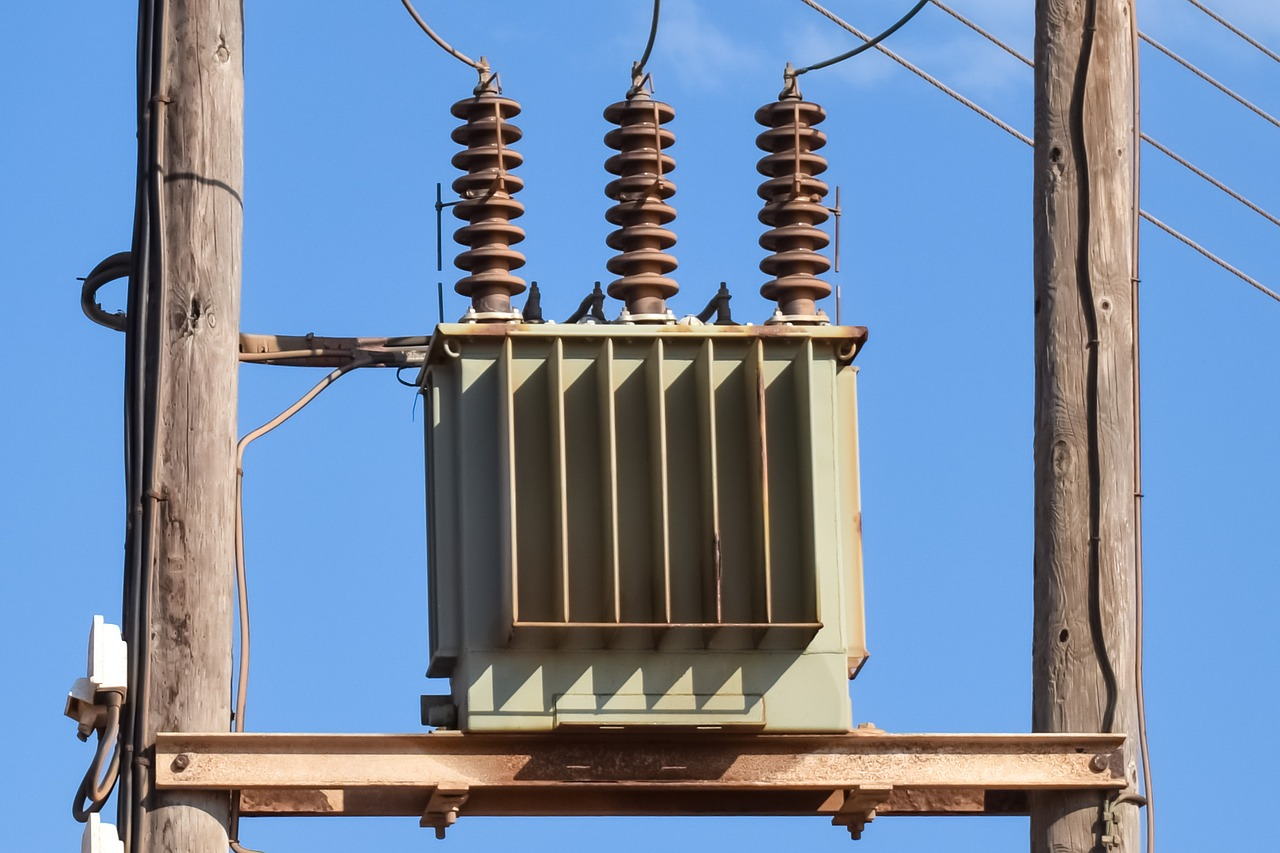
\includegraphics[width=0.5\linewidth]{Images/Trafo.png}
            \caption{Distribution transformer on an electric post.}
            \label{fig:Trafo}
        \end{figure}
    \end{columns}
    \pause
    \begin{alertblock}{Limitations}
        Integration of renewable energy sources is expected to increase. This may cause voltage fluctuations and power quality issues. Conventional DTs are not suitable for a future grid.
    \end{alertblock}
\end{frame}

\subsection{SSTs}

\begin{frame}{Solid-State Transformers}
    \begin{columns}
        \column{0.4\textwidth}
            \begin{figure}
                \centering
                \resizebox{!}{1.7cm}{

\tikzset{every picture/.style={line width=0.75pt}} %set default line width to 0.75pt        

\begin{tikzpicture}[x=0.75pt,y=0.75pt,yscale=-1,xscale=1]
%uncomment if require: \path (0,115); %set diagram left start at 0, and has height of 115

%Shape: Rectangle [id:dp9231641505478003] 
\draw  [fill={rgb, 255:red, 255; green, 255; blue, 255 }  ,fill opacity=1 ][general shadow={fill=black,shadow xshift=0.75pt,shadow yshift=-0.75pt}] (168,32) -- (216,32) -- (216,80) -- (168,80) -- cycle ;
%Straight Lines [id:da6181431125937316] 
\draw    (216,32) -- (168,80) ;

%Shape: Rectangle [id:dp596131781198403] 
\draw  [fill={rgb, 255:red, 255; green, 255; blue, 255 }  ,fill opacity=1 ][general shadow={fill=black,shadow xshift=0.75pt,shadow yshift=-0.75pt}] (248,32) -- (296,32) -- (296,80) -- (248,80) -- cycle ;
%Straight Lines [id:da3641681168334696] 
\draw    (296,32) -- (248,80) ;

%Shape: Rectangle [id:dp07548083531206529] 
\draw  [fill={rgb, 255:red, 255; green, 255; blue, 255 }  ,fill opacity=1 ][general shadow={fill=black,shadow xshift=0.75pt,shadow yshift=-0.75pt}] (328,32) -- (376,32) -- (376,80) -- (328,80) -- cycle ;
%Straight Lines [id:da3658367670720164] 
\draw    (376,32) -- (328,80) ;

%Straight Lines [id:da06410574956465687] 
\draw    (216,40) -- (248,40) ;
%Straight Lines [id:da18560373823094123] 
\draw    (216,72) -- (248,72) ;
%Straight Lines [id:da42261704380295817] 
\draw    (296,40) -- (328,40) ;
%Straight Lines [id:da12224611517010664] 
\draw    (296,72) -- (328,72) ;
%Straight Lines [id:da8439794700421153] 
\draw    (376,56) -- (392,56) ;
%Straight Lines [id:da6436066440115817] 
\draw    (152,56) -- (168,56) ;
%Shape: Ellipse [id:dp8684782137349554] 
\draw   (392,56) .. controls (392,49.37) and (397.22,44) .. (403.65,44) .. controls (410.09,44) and (415.3,49.37) .. (415.3,56) .. controls (415.3,62.63) and (410.09,68) .. (403.65,68) .. controls (397.22,68) and (392,62.63) .. (392,56) -- cycle ;
%Curve Lines [id:da2737310247323681] 
\draw    (396.62,55.26) .. controls (403.47,36.78) and (401.8,72.78) .. (410.31,55.64) ;

%Shape: Ellipse [id:dp7418480653399351] 
\draw   (128.7,57) .. controls (128.7,50.37) and (133.91,45) .. (140.35,45) .. controls (146.78,45) and (152,50.37) .. (152,57) .. controls (152,63.63) and (146.78,69) .. (140.35,69) .. controls (133.91,69) and (128.7,63.63) .. (128.7,57) -- cycle ;
%Curve Lines [id:da7971426217328144] 
\draw    (133.32,56.26) .. controls (140.16,37.78) and (138.5,73.78) .. (147.01,56.64) ;


% Text Node
\draw (177,39.29) node  [font=\footnotesize] [align=left] {AC};
% Text Node
\draw (207,72.71) node  [font=\footnotesize] [align=left] {DC};
% Text Node
\draw (287,72.71) node  [font=\footnotesize] [align=left] {DC};
% Text Node
\draw (257,39.29) node  [font=\footnotesize] [align=left] {DC};
% Text Node
\draw (367,72.71) node  [font=\footnotesize] [align=left] {AC};
% Text Node
\draw (337,39.29) node  [font=\footnotesize] [align=left] {DC};
% Text Node
\draw (191.5,97.5) node  [font=\scriptsize] [align=left] {\begin{minipage}[lt]{22.16pt}\setlength\topsep{0pt}
\begin{center}
\textbf{MV}\\\textbf{Stage}
\end{center}

\end{minipage}};
% Text Node
\draw (271.5,94.5) node  [font=\scriptsize] [align=left] {\begin{minipage}[lt]{32.08pt}\setlength\topsep{0pt}
\begin{center}
\textbf{Isolation}\\\textbf{Stage}
\end{center}

\end{minipage}};
% Text Node
\draw (351.5,97.5) node  [font=\scriptsize] [align=left] {\begin{minipage}[lt]{22.16pt}\setlength\topsep{0pt}
\begin{center}
\textbf{LV}\\\textbf{Stage}
\end{center}

\end{minipage}};
% Text Node
\draw (140,86.5) node  [font=\scriptsize] [align=left] {\begin{minipage}[lt]{16.21pt}\setlength\topsep{0pt}
\begin{center}
MV\\Grid
\end{center}

\end{minipage}};
% Text Node
\draw (404,81.5) node  [font=\scriptsize] [align=left] {\begin{minipage}[lt]{16.21pt}\setlength\topsep{0pt}
\begin{center}
LV\\Grid
\end{center}

\end{minipage}};


\end{tikzpicture}}
                \caption{Solid-state Transformer.}
                \label{fig:HDT}
            \end{figure}
        \column{0.6\textwidth}
            \begin{itemize}
            \item To overcome the limitations of DTs, solid-state transformers (SSTs) have been proposed.
            \begin{itemize}
                \item These devices are based either a AC-AC converter or a AC-DC/DC-AC converter with a active rectifier for the DC stage.
            \end{itemize}
            \item SSTs replace the conventional DT with a fully rated power converter.
            \begin{itemize}
                \item This provides a regulated voltage for a connected load while it's working in full-load operation.
            \end{itemize}
        \end{itemize}
    \end{columns}
    \pause
    \begin{alertblock}{Limitations}
        However, this solution is complex, costly, and offers limited short-circuit capability.
    \end{alertblock}
\end{frame}

\subsection{HDT as a Promising Solution}

\begin{frame}{Hybrid Distribution Transformers}
    \begin{columns}
        \column{0.6\textwidth}
            \begin{itemize}
                \item To address the limitations of both DTs and SSTs, hybrid distribution transformers (HDTs) have emerged as a promising solution.
                \begin{itemize}
                    \item HDTs integrate a traditional DT with a power electronics converter.
                    \item The most common HDT configuration features a series converter for voltage regulation and a parallel converter for current-based power quality compensation.
                    \item The DT handles the majority of the power flow efficiently, leveraging its inherent strengths.
                \end{itemize}
            \end{itemize}
        \column{0.4\textwidth}
            \begin{figure}
                \centering
                \resizebox{!}{5.3cm}{

\tikzset{every picture/.style={line width=0.75pt}} %set default line width to 0.75pt        

\begin{tikzpicture}[x=0.75pt,y=0.75pt,yscale=-1,xscale=1]
%uncomment if require: \path (0,281); %set diagram left start at 0, and has height of 281

%Rounded Rect [id:dp1498416922615955] 
\draw  [fill={rgb, 255:red, 255; green, 0; blue, 0 }  ,fill opacity=0.2 ] (48,135.75) .. controls (48,131.47) and (51.47,128) .. (55.75,128) -- (184.25,128) .. controls (188.53,128) and (192,131.47) .. (192,135.75) -- (192,248.25) .. controls (192,252.53) and (188.53,256) .. (184.25,256) -- (55.75,256) .. controls (51.47,256) and (48,252.53) .. (48,248.25) -- cycle ;
%Shape: Triangle [id:dp46443946003277636] 
\draw  [fill={rgb, 255:red, 255; green, 255; blue, 255 }  ,fill opacity=1 ] (119.41,63.91) -- (95.81,87.95) -- (95.81,39.87) -- cycle ;
%Shape: Polygon [id:ds8300633911306601] 
\draw  [fill={rgb, 255:red, 255; green, 255; blue, 255 }  ,fill opacity=1 ][general shadow={fill=black,shadow xshift=0.75pt,shadow yshift=-0.75pt}] (143,39.87) -- (143,87.95) -- (97.29,87.95) -- (120.88,63.91) -- (97.29,39.87) -- cycle ;
%Straight Lines [id:da7060653075357857] 
\draw    (120.88,63.91) -- (143,63.91) ;

%Straight Lines [id:da6363435803598962] 
\draw    (64,64) -- (96,64) ;
%Straight Lines [id:da5267996923036957] 
\draw    (120,88) -- (120,108) ;
%Straight Lines [id:da44726021460361265] 
\draw    (120,8) -- (120,40) ;
%Straight Lines [id:da668258115881776] 
\draw    (95.81,87.95) -- (56,128) ;
%Straight Lines [id:da9214301838509702] 
\draw    (144,88) -- (184,128) ;
%Shape: Inductor (Air Core) [id:dp83632344975283] 
\draw   (88,152) -- (83.68,152) .. controls (83.68,153.77) and (82.82,155.2) .. (81.76,155.2) .. controls (80.7,155.2) and (79.84,153.77) .. (79.84,152) .. controls (79.84,153.77) and (78.98,155.2) .. (77.92,155.2) .. controls (76.86,155.2) and (76,153.77) .. (76,152) .. controls (76,153.77) and (75.14,155.2) .. (74.08,155.2) .. controls (73.02,155.2) and (72.16,153.77) .. (72.16,152) .. controls (72.16,153.77) and (71.3,155.2) .. (70.24,155.2) .. controls (69.18,155.2) and (68.32,153.77) .. (68.32,152) -- (64,152) ;
%Shape: Inductor (Air Core) [id:dp7999508751202471] 
\draw   (64,168) -- (68.32,168) .. controls (68.32,166.23) and (69.18,164.8) .. (70.24,164.8) .. controls (71.3,164.8) and (72.16,166.23) .. (72.16,168) .. controls (72.16,166.23) and (73.02,164.8) .. (74.08,164.8) .. controls (75.14,164.8) and (76,166.23) .. (76,168) .. controls (76,166.23) and (76.86,164.8) .. (77.92,164.8) .. controls (78.98,164.8) and (79.84,166.23) .. (79.84,168) .. controls (79.84,166.23) and (80.7,164.8) .. (81.76,164.8) .. controls (82.82,164.8) and (83.68,166.23) .. (83.68,168) -- (88,168) ;
%Straight Lines [id:da8313103681431602] 
\draw    (85,158.4) -- (67,158.4) ;
%Straight Lines [id:da41157882719633565] 
\draw    (85,161.6) -- (67,161.6) ;

%Shape: Ellipse [id:dp9743148466945699] 
\draw  [fill={rgb, 255:red, 255; green, 255; blue, 255 }  ,fill opacity=1 ] (108.32,152) .. controls (108.32,147.58) and (111.81,144) .. (116.11,144) .. controls (120.41,144) and (123.89,147.58) .. (123.89,152) .. controls (123.89,156.42) and (120.41,160) .. (116.11,160) .. controls (111.81,160) and (108.32,156.42) .. (108.32,152) -- cycle ;
%Straight Lines [id:da3385079185306148] 
\draw    (88,152) -- (108.32,152) ;
%Shape: Ellipse [id:dp4056578022596924] 
\draw  [fill={rgb, 255:red, 255; green, 255; blue, 255 }  ,fill opacity=1 ] (120,152) .. controls (120,147.58) and (123.48,144) .. (127.78,144) .. controls (132.08,144) and (135.57,147.58) .. (135.57,152) .. controls (135.57,156.42) and (132.08,160) .. (127.78,160) .. controls (123.48,160) and (120,156.42) .. (120,152) -- cycle ;
%Shape: Rectangle [id:dp5537843893958982] 
\draw  [fill={rgb, 255:red, 255; green, 255; blue, 255 }  ,fill opacity=1 ][general shadow={fill=black,shadow xshift=0.75pt,shadow yshift=-0.75pt}] (88.23,200.51) -- (111.09,200.51) -- (111.09,223.76) -- (88.23,223.76) -- cycle ;
%Straight Lines [id:da45439810694201177] 
\draw    (111.09,200.51) -- (88.23,223.76) ;

%Shape: Rectangle [id:dp3659605277693705] 
\draw  [fill={rgb, 255:red, 255; green, 255; blue, 255 }  ,fill opacity=1 ][general shadow={fill=black,shadow xshift=0.75pt,shadow yshift=-0.75pt}] (136.55,200.51) -- (159.66,200.51) -- (159.66,223.76) -- (136.55,223.76) -- cycle ;
%Straight Lines [id:da9862335388880625] 
\draw    (159.66,200.51) -- (136.55,223.76) ;

%Straight Lines [id:da8530054247718197] 
\draw    (76,172) -- (76,212) -- (87.68,212) ;
%Shape: Capacitor [id:dp052526262560992576] 
\draw   (127.57,204) -- (127.57,211.2) (131.46,212.8) -- (123.68,212.8) (131.46,211.2) -- (123.68,211.2) (127.57,212.8) -- (127.57,220) ;
%Straight Lines [id:da06685240362324807] 
\draw    (112,204) -- (128,204) ;
\draw [shift={(128,204)}, rotate = 0] [color={rgb, 255:red, 0; green, 0; blue, 0 }  ][fill={rgb, 255:red, 0; green, 0; blue, 0 }  ][line width=0.75]      (0, 0) circle [x radius= 1.34, y radius= 1.34]   ;
%Straight Lines [id:da08687878975255625] 
\draw    (128,204) -- (136,204) ;
%Straight Lines [id:da05664366026061396] 
\draw    (112,220) -- (127.57,220) ;
\draw [shift={(127.57,220)}, rotate = 0] [color={rgb, 255:red, 0; green, 0; blue, 0 }  ][fill={rgb, 255:red, 0; green, 0; blue, 0 }  ][line width=0.75]      (0, 0) circle [x radius= 1.34, y radius= 1.34]   ;
%Straight Lines [id:da18202214085786328] 
\draw    (127.57,220) -- (136,220) ;
%Straight Lines [id:da8257196245918859] 
\draw    (172,152) -- (172,212) -- (160,212) ;
\draw [shift={(172,152)}, rotate = 90] [color={rgb, 255:red, 0; green, 0; blue, 0 }  ][fill={rgb, 255:red, 0; green, 0; blue, 0 }  ][line width=0.75]      (0, 0) circle [x radius= 1.34, y radius= 1.34]   ;
%Straight Lines [id:da15625609577334676] 
\draw    (135.57,152) -- (176.43,152) ;
%Straight Lines [id:da7061059641709855] 
\draw    (50.35,152) -- (64,152) ;
\draw [shift={(48,152)}, rotate = 0] [color={rgb, 255:red, 0; green, 0; blue, 0 }  ][line width=0.75]      (0, 0) circle [x radius= 3.35, y radius= 3.35]   ;
%Straight Lines [id:da7563615687380554] 
\draw    (176.43,152) -- (189.65,152) ;
\draw [shift={(192,152)}, rotate = 0] [color={rgb, 255:red, 0; green, 0; blue, 0 }  ][line width=0.75]      (0, 0) circle [x radius= 3.35, y radius= 3.35]   ;
%Straight Lines [id:da9257628912880724] 
\draw    (120,204) -- (120,253.65) ;
\draw [shift={(120,256)}, rotate = 90] [color={rgb, 255:red, 0; green, 0; blue, 0 }  ][line width=0.75]      (0, 0) circle [x radius= 3.35, y radius= 3.35]   ;
%Shape: Simple Switch [id:dp3562117821380484] 
\draw   (68,148) -- (71.2,148) (80.8,148) -- (84,148) (72.48,147.75) -- (80.16,143.98) (79.52,148) .. controls (79.52,147.58) and (79.81,147.25) .. (80.16,147.25) .. controls (80.51,147.25) and (80.8,147.58) .. (80.8,148) .. controls (80.8,148.42) and (80.51,148.75) .. (80.16,148.75) .. controls (79.81,148.75) and (79.52,148.42) .. (79.52,148) -- cycle (71.2,148) .. controls (71.2,147.58) and (71.49,147.25) .. (71.84,147.25) .. controls (72.19,147.25) and (72.48,147.58) .. (72.48,148) .. controls (72.48,148.42) and (72.19,148.75) .. (71.84,148.75) .. controls (71.49,148.75) and (71.2,148.42) .. (71.2,148) -- cycle ;
%Straight Lines [id:da8570241382152515] 
\draw    (68,148) -- (64,148) -- (64,152) ;
\draw [shift={(64,152)}, rotate = 90] [color={rgb, 255:red, 0; green, 0; blue, 0 }  ][fill={rgb, 255:red, 0; green, 0; blue, 0 }  ][line width=0.75]      (0, 0) circle [x radius= 1.34, y radius= 1.34]   ;
%Straight Lines [id:da8968836011702404] 
\draw    (84,148) -- (88,148) -- (88,152) ;
\draw [shift={(88,152)}, rotate = 90] [color={rgb, 255:red, 0; green, 0; blue, 0 }  ][fill={rgb, 255:red, 0; green, 0; blue, 0 }  ][line width=0.75]      (0, 0) circle [x radius= 1.34, y radius= 1.34]   ;

% Text Node
\draw (119.75,1.5) node  [font=\small] [align=left] {\textbf{LV-AC}};
% Text Node
\draw (120,117.5) node  [font=\small] [align=left] {\textbf{LV-DC}};
% Text Node
\draw (41,54.5) node [anchor=west] [inner sep=0.75pt]  [font=\small] [align=left] {\textbf{MV-DC}};
% Text Node
\draw (134.5,47.5) node  [font=\scriptsize] [align=left] {AC};
% Text Node
\draw (105.5,63.5) node  [font=\scriptsize] [align=left] {AC};
% Text Node
\draw (134.5,80.5) node  [font=\scriptsize] [align=left] {DC};
% Text Node
\draw (116.05,152) node  [font=\tiny]  {$\Delta $};
% Text Node
\draw (127.7,152) node  [font=\tiny]  {$Y$};
% Text Node
\draw (95.14,205.5) node  [font=\tiny] [align=left] {AC};
% Text Node
\draw (104.35,218.5) node  [font=\tiny] [align=left] {DC};
% Text Node
\draw (152.86,218.5) node  [font=\tiny] [align=left] {AC};
% Text Node
\draw (143.54,205.5) node  [font=\tiny] [align=left] {DC};
% Text Node
\draw (82.5,237.5) node  [font=\tiny] [align=left] {Voltage Controlled\\Power Converter};
% Text Node
\draw (158,237.5) node  [font=\tiny] [align=left] {Current Controller\\Power Converter};
% Text Node
\draw (122.5,194.5) node  [font=\tiny] [align=left] {DC-Link};
% Text Node
\draw (48.62,142.5) node [anchor=west] [inner sep=0.75pt]  [font=\tiny] [align=left] {\textbf{MV-AC}};
% Text Node
\draw (191.35,145.5) node [anchor=east] [inner sep=0.75pt]  [font=\tiny] [align=left] {\textbf{LV-AC}};
% Text Node
\draw (120,265.5) node  [font=\tiny] [align=left] {\textbf{LV-DC}};


\end{tikzpicture}}
                \caption{Hybrid distribution Transformer.}
                \label{fig:HDT}
            \end{figure}
    \end{columns}
\end{frame}

\begin{frame}{Drawbacks of HDTs}
    \begin{itemize}
        \item Coupling transformers (CTs), because of its saturation curve, cannot handle fast varying compensation voltages.
        \item Circulating Active Power Flow (CAPF) between main DT and the power converter impoverish the efficiency.
    \end{itemize}
    \begin{exampleblock}{Remarks}
        \begin{itemize}
            \item CAPF can be eliminated by connecting a DC source to the HDT.
            \item Using a HDT as an interlinking converter for a hybrid AC-DC microgrid is a natural method to eliminate CAPF.
        \end{itemize}
    \end{exampleblock}
\end{frame}

\begin{frame}{HDTs as a Promising Solution for AC and DC Microgrids Integration}
    \begin{figure}
        \centering
        \resizebox{!}{5.3cm}{

\tikzset{every picture/.style={line width=0.75pt}} %set default line width to 0.75pt        

\begin{tikzpicture}[x=0.75pt,y=0.75pt,yscale=-1,xscale=1]
%uncomment if require: \path (0,315); %set diagram left start at 0, and has height of 315

%Shape: Rectangle [id:dp36299639453955] 
\draw  [color={rgb, 255:red, 255; green, 0; blue, 0 }  ,draw opacity=1 ][fill={rgb, 255:red, 255; green, 0; blue, 0 }  ,fill opacity=0.25 ][dash pattern={on 4.5pt off 4.5pt}] (88,133) .. controls (88,130.24) and (90.24,128) .. (93,128) -- (187,128) .. controls (189.76,128) and (192,130.24) .. (192,133) -- (192,171) .. controls (192,173.76) and (189.76,176) .. (187,176) -- (93,176) .. controls (90.24,176) and (88,173.76) .. (88,171) -- cycle ;
%Shape: Rectangle [id:dp09007032268016424] 
\draw  [color={rgb, 255:red, 126; green, 211; blue, 33 }  ,draw opacity=1 ][fill={rgb, 255:red, 126; green, 211; blue, 33 }  ,fill opacity=0.25 ] (200,21) .. controls (200,18.24) and (202.24,16) .. (205,16) -- (243,16) .. controls (245.76,16) and (248,18.24) .. (248,21) -- (248,51) .. controls (248,53.76) and (245.76,56) .. (243,56) -- (205,56) .. controls (202.24,56) and (200,53.76) .. (200,51) -- cycle ;
%Shape: Rectangle [id:dp7538822078187675] 
\draw  [color={rgb, 255:red, 80; green, 227; blue, 194 }  ,draw opacity=1 ][fill={rgb, 255:red, 80; green, 227; blue, 194 }  ,fill opacity=0.25 ] (144,21) .. controls (144,18.24) and (146.24,16) .. (149,16) -- (187,16) .. controls (189.76,16) and (192,18.24) .. (192,21) -- (192,51) .. controls (192,53.76) and (189.76,56) .. (187,56) -- (149,56) .. controls (146.24,56) and (144,53.76) .. (144,51) -- cycle ;
%Shape: Rectangle [id:dp38254314765596953] 
\draw   (152,32) -- (184,32) -- (184,48) -- (152,48) -- cycle ;
%Shape: Rectangle [id:dp40775062639027393] 
\draw  [fill={rgb, 255:red, 0; green, 0; blue, 0 }  ,fill opacity=1 ] (154,30) -- (158,30) -- (158,32) -- (154,32) -- cycle ;
%Shape: Rectangle [id:dp8484922427356605] 
\draw  [fill={rgb, 255:red, 0; green, 0; blue, 0 }  ,fill opacity=1 ] (178,30) -- (182,30) -- (182,32) -- (178,32) -- cycle ;
%Straight Lines [id:da9811935771636653] 
\draw    (154,36) -- (158,36) ;
%Straight Lines [id:da23592258919271258] 
\draw    (178,36) -- (182,36) ;
%Straight Lines [id:da17310904483441059] 
\draw    (180,34) -- (180,38) ;


%Shape: Rectangle [id:dp608370505344022] 
\draw  [color={rgb, 255:red, 245; green, 166; blue, 35 }  ,draw opacity=1 ][fill={rgb, 255:red, 245; green, 166; blue, 35 }  ,fill opacity=0.25 ] (88,21) .. controls (88,18.24) and (90.24,16) .. (93,16) -- (131,16) .. controls (133.76,16) and (136,18.24) .. (136,21) -- (136,51) .. controls (136,53.76) and (133.76,56) .. (131,56) -- (93,56) .. controls (90.24,56) and (88,53.76) .. (88,51) -- cycle ;
%Shape: Parallelogram [id:dp5542004190325218] 
\draw  [fill={rgb, 255:red, 0; green, 0; blue, 255 }  ,fill opacity=0.25 ] (100.1,24) -- (132,24) -- (123.9,40) -- (92,40) -- cycle ;
%Straight Lines [id:da5044587363845592] 
\draw    (96,40) -- (100,32) ;
%Straight Lines [id:da007739550083210478] 
\draw    (100,40) -- (104,32) ;
%Straight Lines [id:da8618146610691602] 
\draw    (104,40) -- (108,32) ;
%Straight Lines [id:da3063231199330758] 
\draw    (108,40) -- (112,32) ;
%Straight Lines [id:da3873698645587713] 
\draw    (112,40) -- (116,32) ;
%Straight Lines [id:da07382503135839613] 
\draw    (116,40) -- (120,32) ;
%Straight Lines [id:da6307749528038389] 
\draw    (120,40) -- (124,32) ;
%Straight Lines [id:da7078011067031311] 
\draw    (94,36) -- (126,36) ;
%Straight Lines [id:da36003974470731626] 
\draw    (100,32) -- (104,24) ;
%Straight Lines [id:da6574946945911684] 
\draw    (104,32) -- (108,24) ;
%Straight Lines [id:da6630449731731625] 
\draw    (108,32) -- (112,24) ;
%Straight Lines [id:da7804944245776355] 
\draw    (112,32) -- (116,24) ;
%Straight Lines [id:da8297470482526796] 
\draw    (116,32) -- (120,24) ;
%Straight Lines [id:da7048240489300945] 
\draw    (120,32) -- (124,24) ;
%Straight Lines [id:da9645536648637945] 
\draw    (124,32) -- (128,24) ;
%Straight Lines [id:da4231587866518627] 
\draw    (98,28) -- (130,28) ;
%Shape: Rectangle [id:dp49159466073928093] 
\draw  [fill={rgb, 255:red, 0; green, 0; blue, 0 }  ,fill opacity=1 ] (100,46) -- (124,46) -- (124,48) -- (100,48) -- cycle ;
%Shape: Rectangle [id:dp9010988432626634] 
\draw  [fill={rgb, 255:red, 0; green, 0; blue, 0 }  ,fill opacity=1 ] (110,40) -- (114,40) -- (114,46) -- (110,46) -- cycle ;
%Straight Lines [id:da18563016734416338] 
\draw    (96,32) -- (128,32) ;

%Shape: Rectangle [id:dp5266278023932072] 
\draw  [fill={rgb, 255:red, 255; green, 255; blue, 255 }  ,fill opacity=1 ][general shadow={fill=black,shadow xshift=0.75pt,shadow yshift=-0.75pt}] (95.85,64.53) -- (128,64.53) -- (128,96) -- (95.85,96) -- cycle ;
%Straight Lines [id:da09304750451052368] 
\draw    (128,64) -- (95.85,97.3) ;

%Straight Lines [id:da17655468696959464] 
\draw [line width=2.25]    (72,112) -- (256,112) ;
%Shape: Ellipse [id:dp7656190687221771] 
\draw   (41,152) .. controls (41,145.37) and (46.22,140) .. (52.65,140) .. controls (59.09,140) and (64.3,145.37) .. (64.3,152) .. controls (64.3,158.63) and (59.09,164) .. (52.65,164) .. controls (46.22,164) and (41,158.63) .. (41,152) -- cycle ;
%Curve Lines [id:da6261869691155981] 
\draw    (45.62,151.26) .. controls (52.47,132.78) and (50.8,168.78) .. (59.31,151.64) ;

%Straight Lines [id:da8271638976646392] 
\draw    (112,56) -- (112,64) ;
%Shape: Rectangle [id:dp4100675503446629] 
\draw  [fill={rgb, 255:red, 255; green, 255; blue, 255 }  ,fill opacity=1 ][general shadow={fill=black,shadow xshift=0.75pt,shadow yshift=-0.75pt}] (152,64.53) -- (184.15,64.53) -- (184.15,96) -- (152,96) -- cycle ;
%Straight Lines [id:da6292272341172389] 
\draw    (184.15,64) -- (152,97.3) ;

%Straight Lines [id:da12174681331026616] 
\draw    (168,56) -- (168,64) ;
%Straight Lines [id:da4329994692833059] 
\draw    (112,96) -- (112,112) ;
\draw [shift={(112,112)}, rotate = 90] [color={rgb, 255:red, 0; green, 0; blue, 0 }  ][fill={rgb, 255:red, 0; green, 0; blue, 0 }  ][line width=0.75]      (0, 0) circle [x radius= 2.01, y radius= 2.01]   ;
%Straight Lines [id:da5644216395705126] 
\draw    (168,96) -- (168,112) ;
\draw [shift={(168,112)}, rotate = 90] [color={rgb, 255:red, 0; green, 0; blue, 0 }  ][fill={rgb, 255:red, 0; green, 0; blue, 0 }  ][line width=0.75]      (0, 0) circle [x radius= 2.01, y radius= 2.01]   ;
%Shape: Path Data [id:dp9539730007897249] 
\draw  [fill={rgb, 255:red, 245; green, 166; blue, 35 }  ,fill opacity=0.25 ] (240,48) -- (228,48) -- (228,40) -- (220,40) -- (220,48) -- (208,48) -- (208,32) -- (224,24) -- (240,32) -- (240,48) -- cycle ;
%Straight Lines [id:da8603794313537159] 
\draw    (204,32) -- (224,22) ;
%Straight Lines [id:da8962214948125011] 
\draw    (224,22) -- (244,32) ;
%Shape: Rectangle [id:dp453727161992874] 
\draw  [fill={rgb, 255:red, 0; green, 0; blue, 0 }  ,fill opacity=1 ] (236,24) -- (238,24) -- (238,30) -- (236,30) -- cycle ;

%Straight Lines [id:da5355085247991662] 
\draw    (224,56) -- (224,112) ;
\draw [shift={(224,112)}, rotate = 90] [color={rgb, 255:red, 0; green, 0; blue, 0 }  ][fill={rgb, 255:red, 0; green, 0; blue, 0 }  ][line width=0.75]      (0, 0) circle [x radius= 2.01, y radius= 2.01]   ;
%Shape: Rectangle [id:dp38730832406139215] 
\draw  [color={rgb, 255:red, 126; green, 211; blue, 33 }  ,draw opacity=1 ][fill={rgb, 255:red, 126; green, 211; blue, 33 }  ,fill opacity=0.25 ] (200,253) .. controls (200,250.24) and (202.24,248) .. (205,248) -- (243,248) .. controls (245.76,248) and (248,250.24) .. (248,253) -- (248,283) .. controls (248,285.76) and (245.76,288) .. (243,288) -- (205,288) .. controls (202.24,288) and (200,285.76) .. (200,283) -- cycle ;
%Shape: Circle [id:dp8211119558841091] 
\draw   (206,262) .. controls (206,258.69) and (208.69,256) .. (212,256) .. controls (215.31,256) and (218,258.69) .. (218,262) .. controls (218,265.31) and (215.31,268) .. (212,268) .. controls (208.69,268) and (206,265.31) .. (206,262) -- cycle ;
%Shape: Circle [id:dp9453082981808478] 
\draw   (208,261) .. controls (208,260.45) and (208.45,260) .. (209,260) .. controls (209.55,260) and (210,260.45) .. (210,261) .. controls (210,261.55) and (209.55,262) .. (209,262) .. controls (208.45,262) and (208,261.55) .. (208,261) -- cycle ;
%Shape: Circle [id:dp4615825814572241] 
\draw   (214,261) .. controls (214,260.45) and (214.45,260) .. (215,260) .. controls (215.55,260) and (216,260.45) .. (216,261) .. controls (216,261.55) and (215.55,262) .. (215,262) .. controls (214.45,262) and (214,261.55) .. (214,261) -- cycle ;
%Shape: Circle [id:dp07473702214392075] 
\draw   (211,265) .. controls (211,264.45) and (211.45,264) .. (212,264) .. controls (212.55,264) and (213,264.45) .. (213,265) .. controls (213,265.55) and (212.55,266) .. (212,266) .. controls (211.45,266) and (211,265.55) .. (211,265) -- cycle ;

%Shape: Rectangle [id:dp13930109452257633] 
\draw   (224,256) -- (240,256) -- (240,280) -- (224,280) -- cycle ;
%Curve Lines [id:da2056385298136112] 
\draw    (212,268) .. controls (209.25,278.92) and (220.45,285.69) .. (224,264) ;
%Shape: Rectangle [id:dp8504838713938807] 
\draw  [fill={rgb, 255:red, 155; green, 155; blue, 155 }  ,fill opacity=1 ] (210,268) -- (214,268) -- (214,274) -- (210,274) -- cycle ;
%Shape: Rectangle [id:dp5317465538337975] 
\draw  [fill={rgb, 255:red, 255; green, 0; blue, 0 }  ,fill opacity=0.25 ] (226,258) -- (238,258) -- (238,264) -- (226,264) -- cycle ;

%Shape: Rectangle [id:dp3203086254752263] 
\draw  [color={rgb, 255:red, 80; green, 227; blue, 194 }  ,draw opacity=1 ][fill={rgb, 255:red, 80; green, 227; blue, 194 }  ,fill opacity=0.25 ] (144,253) .. controls (144,250.24) and (146.24,248) .. (149,248) -- (187,248) .. controls (189.76,248) and (192,250.24) .. (192,253) -- (192,283) .. controls (192,285.76) and (189.76,288) .. (187,288) -- (149,288) .. controls (146.24,288) and (144,285.76) .. (144,283) -- cycle ;
%Shape: Rectangle [id:dp2653700015147502] 
\draw   (152,264) -- (184,264) -- (184,280) -- (152,280) -- cycle ;
%Shape: Rectangle [id:dp8930820672294637] 
\draw  [fill={rgb, 255:red, 0; green, 0; blue, 0 }  ,fill opacity=1 ] (154,262) -- (158,262) -- (158,264) -- (154,264) -- cycle ;
%Shape: Rectangle [id:dp5896749728034121] 
\draw  [fill={rgb, 255:red, 0; green, 0; blue, 0 }  ,fill opacity=1 ] (178,262) -- (182,262) -- (182,264) -- (178,264) -- cycle ;
%Straight Lines [id:da7887351195081793] 
\draw    (154,268) -- (158,268) ;
%Straight Lines [id:da5561146518517932] 
\draw    (178,268) -- (182,268) ;
%Straight Lines [id:da7643548865379168] 
\draw    (180,266) -- (180,270) ;


%Shape: Rectangle [id:dp3575939081610673] 
\draw  [color={rgb, 255:red, 245; green, 166; blue, 35 }  ,draw opacity=1 ][fill={rgb, 255:red, 245; green, 166; blue, 35 }  ,fill opacity=0.25 ] (88,253) .. controls (88,250.24) and (90.24,248) .. (93,248) -- (131,248) .. controls (133.76,248) and (136,250.24) .. (136,253) -- (136,283) .. controls (136,285.76) and (133.76,288) .. (131,288) -- (93,288) .. controls (90.24,288) and (88,285.76) .. (88,283) -- cycle ;
%Shape: Parallelogram [id:dp8288201139793847] 
\draw  [fill={rgb, 255:red, 0; green, 0; blue, 255 }  ,fill opacity=0.25 ] (100.1,256) -- (132,256) -- (123.9,272) -- (92,272) -- cycle ;
%Straight Lines [id:da23574909008404643] 
\draw    (96,272) -- (100,264) ;
%Straight Lines [id:da4671840220374326] 
\draw    (100,272) -- (104,264) ;
%Straight Lines [id:da5542049138514937] 
\draw    (104,272) -- (108,264) ;
%Straight Lines [id:da45593053792004445] 
\draw    (108,272) -- (112,264) ;
%Straight Lines [id:da5890467686626477] 
\draw    (112,272) -- (116,264) ;
%Straight Lines [id:da7639730134684768] 
\draw    (116,272) -- (120,264) ;
%Straight Lines [id:da6457526609453472] 
\draw    (120,272) -- (124,264) ;
%Straight Lines [id:da4809714694919678] 
\draw    (94,268) -- (126,268) ;
%Straight Lines [id:da6937156244672318] 
\draw    (100,264) -- (104,256) ;
%Straight Lines [id:da5268855450380487] 
\draw    (104,264) -- (108,256) ;
%Straight Lines [id:da45382371701169677] 
\draw    (108,264) -- (112,256) ;
%Straight Lines [id:da40135843513989955] 
\draw    (112,264) -- (116,256) ;
%Straight Lines [id:da8797748031397894] 
\draw    (116,264) -- (120,256) ;
%Straight Lines [id:da5396455589833746] 
\draw    (120,264) -- (124,256) ;
%Straight Lines [id:da016938022936106245] 
\draw    (124,264) -- (128,256) ;
%Straight Lines [id:da948682127834509] 
\draw    (98,260) -- (130,260) ;
%Shape: Rectangle [id:dp08846496054139119] 
\draw  [fill={rgb, 255:red, 0; green, 0; blue, 0 }  ,fill opacity=1 ] (100,278) -- (124,278) -- (124,280) -- (100,280) -- cycle ;
%Shape: Rectangle [id:dp5628333633883209] 
\draw  [fill={rgb, 255:red, 0; green, 0; blue, 0 }  ,fill opacity=1 ] (110,272) -- (114,272) -- (114,278) -- (110,278) -- cycle ;
%Straight Lines [id:da04267186502093012] 
\draw    (96,264) -- (128,264) ;

%Shape: Rectangle [id:dp6894530422096654] 
\draw  [fill={rgb, 255:red, 255; green, 255; blue, 255 }  ,fill opacity=1 ][general shadow={fill=black,shadow xshift=0.75pt,shadow yshift=-0.75pt}] (96,208.53) -- (128.15,208.53) -- (128.15,240) -- (96,240) -- cycle ;
%Straight Lines [id:da6601174977334654] 
\draw    (128.15,208) -- (96,241.3) ;

%Straight Lines [id:da8133837980938741] 
\draw [line width=2.25]    (80,192) -- (256,192) ;
%Straight Lines [id:da429414083050879] 
\draw    (112.15,240) -- (112.15,248) ;
%Shape: Rectangle [id:dp9939560108088266] 
\draw  [fill={rgb, 255:red, 255; green, 255; blue, 255 }  ,fill opacity=1 ][general shadow={fill=black,shadow xshift=0.75pt,shadow yshift=-0.75pt}] (152.15,208.53) -- (184.29,208.53) -- (184.29,240) -- (152.15,240) -- cycle ;
%Straight Lines [id:da31690351887272317] 
\draw    (184.29,208) -- (152.15,241.3) ;

%Straight Lines [id:da4925450690668529] 
\draw    (168.15,240) -- (168.15,248) ;
%Straight Lines [id:da9460906042589992] 
\draw    (112,192) -- (112,208) ;
\draw [shift={(112,192)}, rotate = 90] [color={rgb, 255:red, 0; green, 0; blue, 0 }  ][fill={rgb, 255:red, 0; green, 0; blue, 0 }  ][line width=0.75]      (0, 0) circle [x radius= 2.01, y radius= 2.01]   ;
%Straight Lines [id:da7953255510649611] 
\draw    (168,192) -- (168,208) ;
\draw [shift={(168,192)}, rotate = 90] [color={rgb, 255:red, 0; green, 0; blue, 0 }  ][fill={rgb, 255:red, 0; green, 0; blue, 0 }  ][line width=0.75]      (0, 0) circle [x radius= 2.01, y radius= 2.01]   ;
%Straight Lines [id:da20603228224739278] 
\draw    (224,192) -- (224,208) ;
\draw [shift={(224,192)}, rotate = 90] [color={rgb, 255:red, 0; green, 0; blue, 0 }  ][fill={rgb, 255:red, 0; green, 0; blue, 0 }  ][line width=0.75]      (0, 0) circle [x radius= 2.01, y radius= 2.01]   ;
%Shape: Rectangle [id:dp25752390998743535] 
\draw  [fill={rgb, 255:red, 255; green, 255; blue, 255 }  ,fill opacity=1 ][general shadow={fill=black,shadow xshift=0.75pt,shadow yshift=-0.75pt}] (208,207.23) -- (240.15,207.23) -- (240.15,238.7) -- (208,238.7) -- cycle ;
%Straight Lines [id:da8164804894780389] 
\draw    (240.15,206.7) -- (208,240) ;

%Straight Lines [id:da6013771130407253] 
\draw    (224.15,240) -- (224.15,248) ;
%Straight Lines [id:da8978300902586673] 
\draw    (112,168) -- (112,192) ;
%Straight Lines [id:da006449366621711361] 
\draw    (112,112) -- (112,136) ;
%Shape: Triangle [id:dp12868896874136726] 
\draw  [fill={rgb, 255:red, 255; green, 255; blue, 255 }  ,fill opacity=1 ] (112,152) -- (96,168) -- (96,136) -- cycle ;
%Shape: Polygon [id:ds12605022596129922] 
\draw  [fill={rgb, 255:red, 255; green, 255; blue, 255 }  ,fill opacity=1 ][general shadow={fill=black,shadow xshift=0.75pt,shadow yshift=-0.75pt}] (128,136) -- (128,168) -- (96,168) -- (112,152) -- (96,136) -- cycle ;

%Straight Lines [id:da5721175987893949] 
\draw    (112,152) -- (128,152) ;
%Straight Lines [id:da900039405692058] 
\draw    (96,152) -- (64,152) ;

% Text Node
\draw (52.5,129.5) node  [font=\scriptsize] [align=left] {MV-AC};
% Text Node
\draw (105.5,71.5) node  [font=\scriptsize] [align=left] {DC};
% Text Node
\draw (118.5,88.5) node  [font=\scriptsize] [align=left] {AC};
% Text Node
\draw (174.65,88.5) node  [font=\scriptsize] [align=left] {AC};
% Text Node
\draw (161.65,71.5) node  [font=\scriptsize] [align=left] {DC};
% Text Node
\draw (287.5,112.5) node  [font=\scriptsize] [align=left] {AC Microgrid};
% Text Node
\draw (113,8.5) node  [font=\scriptsize] [align=left] {PV};
% Text Node
\draw (168,8.5) node  [font=\scriptsize] [align=left] {BESS};
% Text Node
\draw (224,8.5) node  [font=\scriptsize] [align=left] {AC Loads};
% Text Node
\draw (288.5,192.5) node  [font=\scriptsize] [align=left] {DC Microgrid};
% Text Node
\draw (112,295.5) node  [font=\scriptsize] [align=left] {PV};
% Text Node
\draw (168,295.5) node  [font=\scriptsize] [align=left] {BESS};
% Text Node
\draw (224,295.5) node  [font=\scriptsize] [align=left] {EV Chargers};
% Text Node
\draw (230.65,231.2) node  [font=\scriptsize] [align=left] {DC};
% Text Node
\draw (217.65,214.2) node  [font=\scriptsize] [align=left] {DC};
% Text Node
\draw (174.79,232.5) node  [font=\scriptsize] [align=left] {DC};
% Text Node
\draw (161.79,215.5) node  [font=\scriptsize] [align=left] {DC};
% Text Node
\draw (118.65,232.5) node  [font=\scriptsize] [align=left] {DC};
% Text Node
\draw (105.65,215.5) node  [font=\scriptsize] [align=left] {DC};
% Text Node
\draw (164.5,150.5) node  [font=\scriptsize] [align=left] {Interlinking\\HDT};
% Text Node
\draw (119.5,141.5) node  [font=\scriptsize] [align=left] {AC};
% Text Node
\draw (103,152.5) node  [font=\tiny] [align=left] {AC};
% Text Node
\draw (119.5,161.5) node  [font=\scriptsize] [align=left] {DC};


\end{tikzpicture}}
        \caption{Integration between AC and DC microgrids through a HDT.}
    \end{figure}
\end{frame}

\section{Research Project Methodology}

\begin{frame}{Research Project Methodology}
    \begin{itemize}
        \item State-of-the-art research will be conducted to analyze existing work related to the topic.
        \item New HDT models will be developed and analyzed.
        \item A local HDT controller will be proposed to ensure robust operation. It will address DC-Link voltage regulation, series voltage compensation, and parallel converter current compensation.
        \item An external control layer will be designed to enable the interlinking operation of the HDT, allowing efficient energy flow management between AC and DC microgrids.
    \end{itemize}
\end{frame}

\begin{frame}{Research Project Methodology (continued)}
    \begin{itemize}
        \item The proposed HDT will be simulated using PLECS software, including:
        \begin{itemize}
            \item Different scenarios, such as balanced, unbalanced, and distorted grid voltage and current operations.
            \item Studies of transitions between grid-connected and islanded modes.
        \end{itemize}
        \item An optimization algorithm for a hybrid microgrid will be designed and simulated using real-time hardware-in-the-loop (RT-HiL).
        \begin{itemize}
            \item The proposed interlinking HDT will be integrated as an element of the microgrid.
            \item The optimization algorithm will serve as a supervisory controller, integrating hierarchical control for the microgrid
        \end{itemize}
    \end{itemize}
\end{frame}

\section{Research Productivity}

\subsection{Authored and Planned Submission Papers}

\begin{frame}{Authored Papers}
    \begin{itemize}
        \item Dave Figueroa, et al.: Distributed Energy Resources with LCL Filter Control and Protection Using Model Predictive Control. \textit{Published and presented at ICA-ACCA 2024, Santiago, Chile.}
    \end{itemize}
    \textbf{To be authored:}
    \begin{itemize}
        \item Dave Figueroa, et al.: Unified MPC for Primary Control of Distributed Energy Resources with LCL Filter under Safety Constraints. \textit{Planned submission to IEEE Journal of Emerging Topics in Power Electronics (JESTPE), Q1 - 2023 Impact Factor = 4.6}\footnotemark[1].
        \item Dave Figueroa, et al.: Validation of a Novel Reconfigurable Partial Power Converter and Optimizer for Photovoltaic Panels. \textit{Planned submission to IEEE Journal of Emerging Topics in Power Electronics (JESTPE).}
    \end{itemize}
    \footnotetext[1]{Taken from Journal Citation Reports - Clarivate. Results for 2023}
\end{frame}

\subsection{Co-authored and Planned Submission Papers}

\begin{frame}{Co-authored Papers}
    \begin{itemize}
        \item Reinier Lopez, \textit{et al.}: Experimental Validation of offset-free  MPC in Voltage Source Inverters for Grid Connected and Microgrids Applications. \textit{Accepted in MDPI Applied Sciences.}
        \item Reinier Lopez, \textit{et al.}: Linear Quadratic Tracker in Multi-agent System. \textit{Published and presented at Industrial Electronics Conference (IECON) - 2024, Chicago, USA.}
    \end{itemize}
    \textbf{To be authored:}
    \begin{itemize}
        \item Ignacio A. Acosta, \textit{et al.}: Deep Neural Network-Based Approximation of Model Predictive Control for Integrating DER Units in AC Microgrids. \textit{Planned submission to IEEE Transactions on Smart Grid (TSG), Q1 - 2023 Impact Factor = 8.6}\footnotemark[1].
        \item Maria Coronel, \textit{et al.}: Exact Sampled-data Models for a class of Electrical Machines.
    \end{itemize}
    \footnotetext[1]{Taken from Journal Citation Reports - Clarivate. Results for 2023}
\end{frame}

\begin{frame}{Conferences Participation}
    \begin{columns}
        \column{0.5\textwidth}
            \begin{itemize}
                \item \textbf{ICA - ACCA 2024}, Santiago, Chile, October 20-23, 2024\\
                Presented the paper: \textit{Distributed Energy Resources with LCL Filter Control and Protection Using Model Predictive Control}
                \item \textbf{IECON 2024}, Chicago, Illinois, November 3-6, 2024.\\
                Presented the paper: \textit{Linear Quadratic Tracker in Multi-agent System}
            \end{itemize}
        \column{0.5\textwidth}
            \begin{figure}
                \centering
                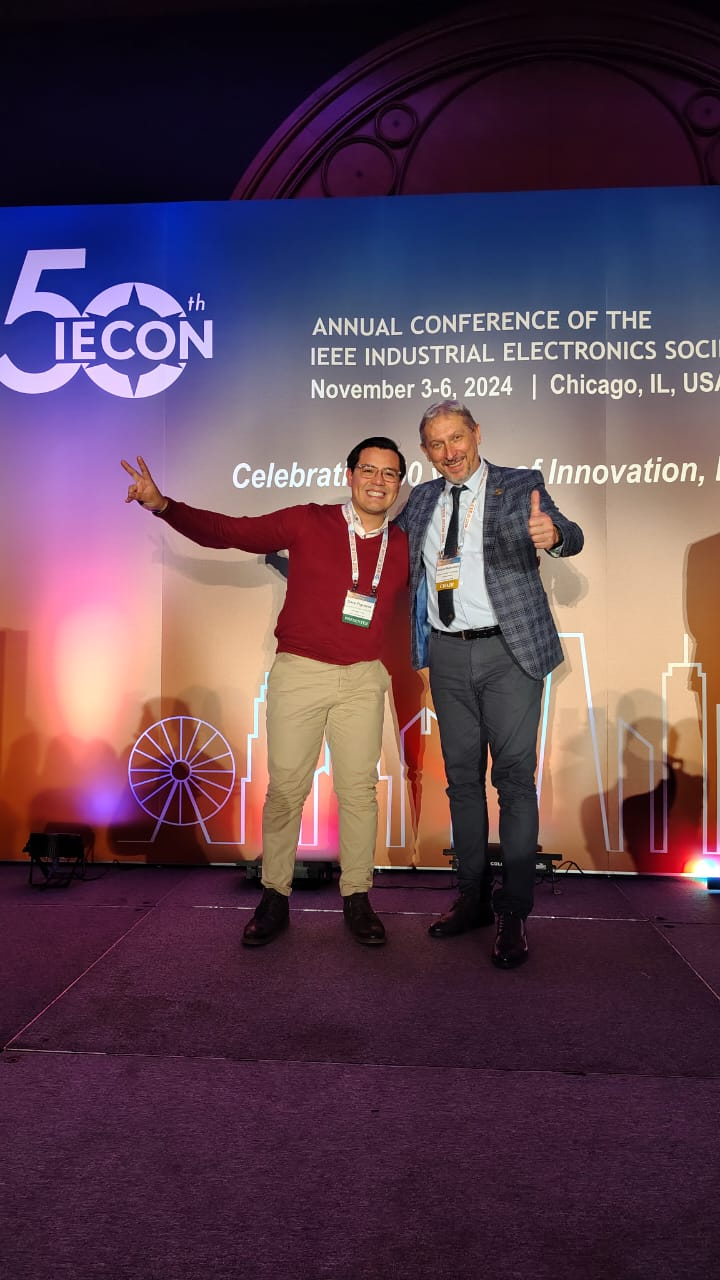
\includegraphics[width=0.45\linewidth]{Images/IECON.jpg}
            \end{figure}
    \end{columns}
\end{frame}

\begin{frame}[plain]
    \setbeamercolor{background canvas}{bg = white}
    \centering \Huge
    \emph{Thanks for your attention}
\end{frame}

\maketitle